\chapter{Analyse der modellprädiktiven Regelung} \label{ch_AnalyseRegelung}
Nachfolgend wird die in Kapitel \ref{ch_Reglerentwurf} vorgestellte Regelung analysiert.
Zunächst wird die genutzte Hard- und Software vorgestellt, bevor anschließend repräsentative Wolkenfälle definiert werden.
Mithilfe eines Referenzszenarios bezüglich der Regelung aus der Literatur kann die Güte der modellprädiktiven Regelung bestimmt werden.
Analysiert wird, ob die thermischen Spannungen der Receiverfront die Grenzwerte überschreiten, wie stark die Temperatur des austretenden Enthalpiestroms bei Wolkeneinfluss vom Referenzwert abweicht und wie hoch der Exergieeintrag in den Folgeprozess ist.
Dabei werden einerseits Simulationen untersucht, bei denen der Regler abweichungsfreie Kenntnis über die Einstrahlung besitzt, sowie andererseits solche, bei denen kein Nowcasting genutzt wird.
Abschließend wird die notwendige Güte der Wolkenvorhersage bezüglich der Wolkengeschwindigkeiten und der Lichtdurchlässigkeit ermittelt.

Die in Jülich vorliegenden Einschränkungen bezüglich der thermischen Maximalbelastungen des Receivers werden dem Betriebshandbuch entnommen (vgl. Kapitel \ref{subsubsec_constraints}).
Dort wird die maximale lokale Temperatur der Absorberfläche, welche direkt von der Flussdichte $\phi$ abhängig ist, mit $\SI{1275.15}{\kelvin}$ angegeben \cite[S.29]{HandbuchJülich}. Dieser Wert dient in den Simulationen als Indikator für eine erfolgreiche Regelung, welche die Einhaltung dieses Limits als Grundvoraussetzung beinhaltet.

\section{Verwendete Hard- und Software} \label{sec_Hardsoftanalyse}
Die in Kapitel \ref{ch_Modellbildung} vorgestellte Modellbildung wird vollständig in do-mpc (siehe Kapitel \ref{sec_HardSoftware}) realisiert und ausgewertet.
Die Berechnung erfolgt mittels der Optimierungssoftware IPOPT (\textbf{I}nterior \textbf{P}oint \textbf{OPT}imizer) in Kombination mit dem HSL ma27 solver.
Aufgrund der Größe des Optimierungsproblems wird die Optimierung nach 100 Iterationsschritten ohne Konvergenz abgebrochen, um die maximale Berechnungsdauer der Optimierung nicht zu überschreiten und quasistatisches Verhalten voraussetzen zu können (vgl. Kapitel \ref{subsubsec_sampletime}).

Die Simulationen werden auf einem 4-Kern Intel Core i7-1185G7 Prozessor mit einem Basistakt von 3,0 GHz durchgeführt.
Als Arbeitsspeicher stehen 16 GB RAM mit 4267 MHz zur Verfügung.
Das Betriebssystem ist Windows 10 Enterprise (Version 21H2).


\section{Repräsentative Wolkenszenarien} \label{sec_reprWolkenszenarien}
Für die Kurzzeitdynamik des Solarturms ist die direkte Verschattung des Heliostatenfeldes durch Wolkendurchzug ausschlaggebend.
Unterschiedliche Wolkengrößen, Zugrichtungen und -geschwindigkeiten haben beliebige zeitliche und räumliche Abschattungsszenarien zur Folge.
Aufgrund des hohen Rechenaufwandes ist die Betrachtung aller real auftretenden Störungen nicht praktikabel.
Stattdessen werden leicht parametrisierbare Störsignale definiert, die zusätzlich eine Vergleichbarkeit mit Ergebnissen anderer Autoren ermöglichen \cite[S.60]{DissHirsch}.

Als Wolkenszenario wird eine einmalige sprungförmige Änderung der Einstrahlung verwendet.
Ein Parameter des Szenarios ist dabei die Intensität des Einstrahlungseinbruches (\textit{shading}).
Diese ist davon abhängig, wie hoch die Lichtdurchlässigkeit der Wolken und der Anteil der verschatteten Heliostaten ist.
Weiterhin ist die Dauer der Verschattung (\textit{duration}) zu definieren; diese beschreibt den Zeitraum zwischen dem Beginn der Verschattung des Heliostatfeldes und dem Beginn des Abklingens dieser Verschattung.
Zuletzt ist auch die Wolkengeschwindigkeit relevant, welche indirekt die Zeitspanne beschreibt, bis die Verschattungsintensität ihr Maximum erreicht (\textit{ramp length}).
In Abbildung \ref{fig_TestszenarioWolken} ist die solare Einstrahlung über der Zeit für ein solches Wolkenszenario mit einer Gesamtabschattung von $\SI{75}{\percent}$ zu sehen.
Diese kann beispielsweise Auftreten, wenn das gesamte Heliostatenfeld verschattet wird und die Lichtdurchlässigkeit der Wolken $\SI{25}{\percent}$ beträgt.

\begin{figure}[h!]
    \centering
    \setlength{\fboxsep}{1pt}
    \setlength{\fboxrule}{1pt}
    \fbox{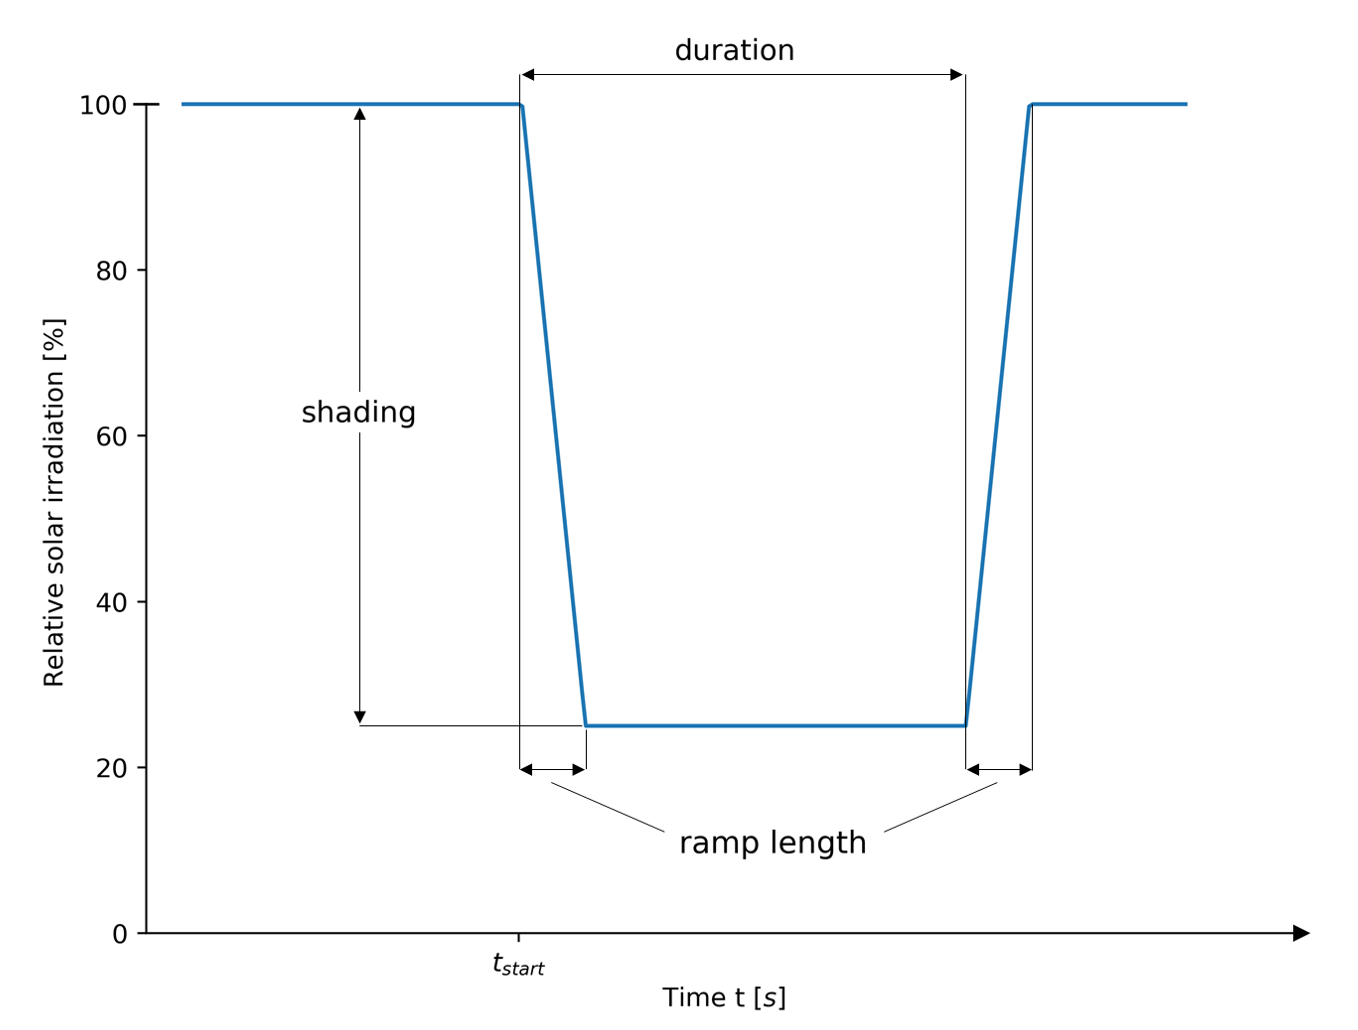
\includegraphics[width=0.92\textwidth]{C:/Users/gesc_ma/VSCode MPC Projekt/dynaovrcontroller/dynaovrcontroller/aimpoint_control_scenarios/plots/23_cloud_scenarios/cloud_sceanrio_clarification_modified.png}}
    \caption[Visualisierung eines beispielhaften Wolkenszenarios]{Visualisierung eines beispielhaften Wolkenszenarios (gemäß \cite[S.62]{DissHirsch})}
    \label{fig_TestszenarioWolken}
\end{figure}

Zur Identifizierung realistischer Wolkenszenarien werden Windmessungen auf der PSA (Plataforma Solar de Almería) in Spanien zur Hilfe genommen.
In Messungen von 2016 und 2017 wurden die Messergebnisse in Gruppen mit einer Breite von $\SI{3}{\metre\per\second}$ eingeteilt.
Die relative Häufigkeit dieser Windgeschwindigkeiten zeigt Abbildung \ref{fig_Windklassen}.

\begin{figure}[h!]
    \centering
    \setlength{\fboxsep}{1pt}
    \setlength{\fboxrule}{1pt}
    \fbox{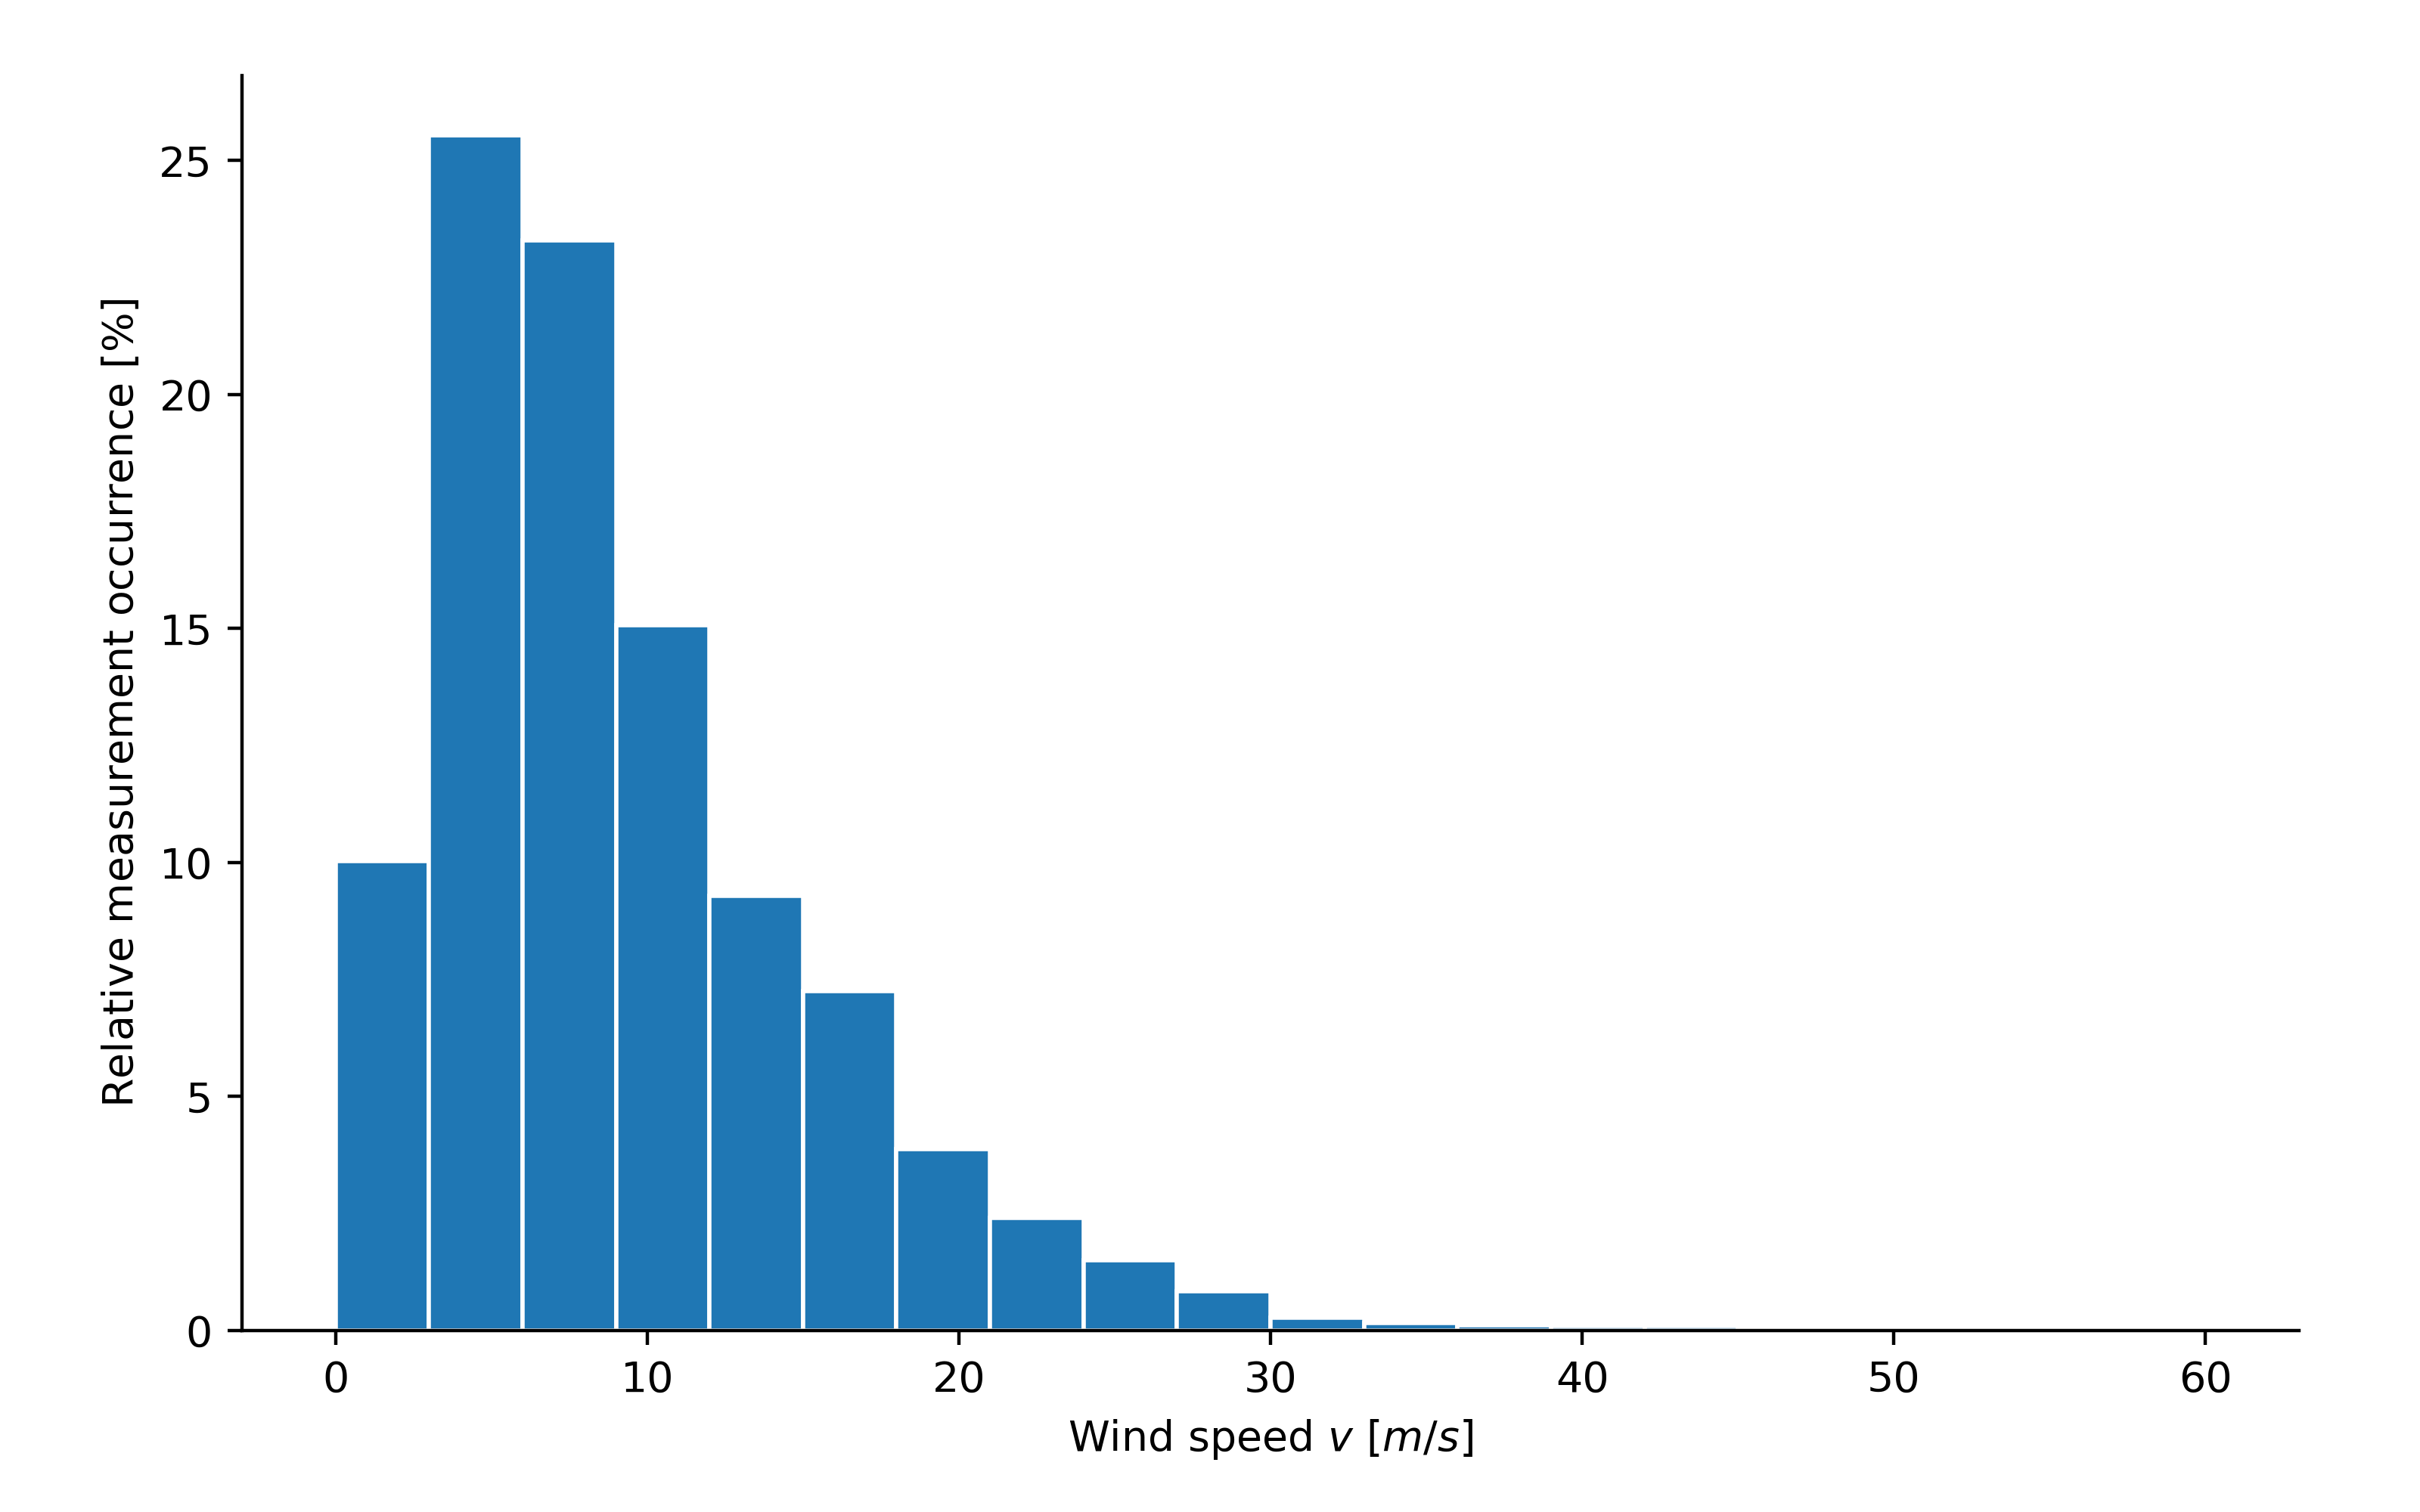
\includegraphics[width=0.99\textwidth]{C:/Users/gesc_ma/VSCode MPC Projekt/dynaovrcontroller/dynaovrcontroller/aimpoint_control_scenarios/plots/23_cloud_scenarios/windspeed_measurements.png}}
    \caption[Relative Häufigkeit der Windgeschwindigkeiten auf der PSA 2016 und 2017]{Relative Häufigkeit der Windgeschwindigkeiten auf der PSA 2016 und 2017}
    \label{fig_Windklassen}
\end{figure}

Um die Regelung nachfolgend bei besonders schnell wechselnden Lichtverhältnissen zu testen, werden Szenarien mit Wolkengeschwindigkeiten von $\SI{15}{\metre\per\second}$, $\SI{20}{\metre\per\second}$, $\SI{25}{\metre\per\second}$ und $\SI{30}{\metre\per\second}$ definiert.
Oberhalb dieser Geschwindigkeiten liegen lediglich $\SI{0.88}{\percent}$ der Windmessungen.
Weiterhin werden Lichtdurchlässigkeiten von $\SI{0}{\percent}$, $\SI{25}{\percent}$, $\SI{50}{\percent}$ und $\SI{75}{\percent}$ untersucht, wobei immer die Abschattung des gesamten Heliostatfeldes angenommen wird.

Die Zugrichtung der Wolken wird in jedem Szenario von Süden nach Norden angenommen.
Wie in Kapitel \ref{subsec_OptimierungZielpunkte} beschrieben, sind die receivernahen Heliostaten besonders zur Fokussierung geeignet.
Durch diese Annahme wird hiermit die kritischste Zugrichtung simuliert, da die fokussierten Heliostaten so eine schnelle Änderung der Einstrahlungsintensität erfahren.
Die Verschattungsdauer wird auf $\SI{120}{\second}$ festgelegt.

\section{Referenzszenario} \label{sec_Referenzszenario}
Als Referenzszenario wird ein sogenanntes \gans{Cloud Standby} Szenraio (nachfolgend CSS genannt) nach dem von Zavoico \cite[S.25ff]{Zavoico} vorgestellten Vorbild eingeführt.
Dieses dient dazu, die Güte der vorgestellten Regelung gegenüber einem in der Literatur erprobten Verfahren einschätzen zu können.
Zavoico beschreibt das Cloud Standby als Szenario, das bei Wolkendurchzug über dem Heliostatenfeld einsetzt.
Dabei werden alle verfügbaren Heliostaten auf vorberechnete Zielpunkte fokussiert und der Massenstrom so eingestellt, dass das Medium bei wolkenlosen Bedingungen mit einer bestimmten Temperatur austreten würde.
Die gewünschte Austrittstemperatur des Mediums bei Wolkendurchzug ist dabei geringer als während des Normalbetriebs.

Das in dieser Arbeit verwendete CSSS unterscheidet sich von dieser Methode dahingehend, dass die Fokussierung der Heliostaten und der Luftmassenstrom gegenüber einem Gleichgewichtszustand bei Normalbetrieb konstant gehalten werden.
Daher wäre mit den Einstellungen zum CSS bei wolkenlosen Bedingungen die identische Austrittstemperatur der Luft zu erwarten wie während regulärer Betriebsbedingungen.

Exemplarisch ist dieser Betriebszustand bei Verschattung um $\SI{50}{\percent}$ bei einer Wolkengeschwindigkeit von $\SI{30}{\metre\per\second}$ in Abbildung \ref{fig_cloudstandby5030} dargestellt.
Da der Einstellwert und die Streuungsfaktoren konstant bleiben, sinkt die Einstrahlungsleistung auf dem Receiver und damit die Fronttemperatur des Absorbers und die Temperatur der austretenden Luft.
Der größte Nachteil dieses Szenarios ist, dass durch die große Abweichung der Temperatur der Austrittsluft gegenüber der Nennlasttemperatur von $\SI{1013.15}{\kelvin}$ \cite[S.29]{HandbuchJülich} der Wirkungsgrad des jeweiligen Folgeprozesses sinkt (vgl. \cite[S.15ff]{DissGall}).
Weiterhin erhöht eine möglichst konstante Temperatur die Langlebigkeit der Komponenten.
Im dargestellten Szenario liegt die Wurzel der mittleren quadratischen Abweichung zwischen Luftaustrittstemperatur und Referenzwert bei $\SI{62.6}{\kelvin}$.

\begin{figure}[h!]
    \centering
    \setlength{\fboxsep}{1pt}
    \setlength{\fboxrule}{1pt}
    \fbox{\includegraphics[width=0.99\textwidth]{C:/Users/gesc_ma/VSCode MPC Projekt/dynaovrcontroller/dynaovrcontroller/aimpoint_control_scenarios/plots/00_no_control/shading_120sec_50_30mps.png}}
\caption[Exemplarischer Simulationsverlauf für das CSS bei Verschattung um $\SI{50}{\percent}$ und $\SI{30}{\metre\per\second}$ Wolkengeschwindigkeit]{Exemplarischer Simulationsverlauf für das CSS bei Verschattung um $\SI{50}{\percent}$ und $\SI{30}{\metre\per\second}$ Wolkengeschwindigkeit}
    \label{fig_cloudstandby5030}
\end{figure}

Abbildung \ref{fig_RMSEcloudstandby} zeigt den RMSE der Temperaturabweichungen für die in Abschnitt \ref{sec_reprWolkenszenarien} festgelegten Wolkenszenarien bezüglich der Lichtdurchlässigkeit und Geschwindigkeit der Wolken.
Es ist erkennbar, dass der RMSE maßgeblich von der Stärke der Verschattung abhängig ist.
Durch die konstanten Systemeingangsgrößen ergibt sich ein nahezu linearer Zusammenhang zwischen Verschattungsintensität und Temperaturabweichung.

\begin{figure}[h!]
    \centering
    \setlength{\fboxsep}{1pt}
    \setlength{\fboxrule}{1pt}
    \fbox{\includegraphics[width=0.99\textwidth]{C:/Users/gesc_ma/VSCode MPC Projekt/dynaovrcontroller/dynaovrcontroller/aimpoint_control_scenarios/plots/22_compare_controller_RMSE/00_no_control.png}}
\caption[Analyse des RMSE der Temperaturabweichungen für das CSS bei unterschiedlichen Wolkenfällen]{Analyse des RMSE der Temperaturabweichungen für das CSS bei unterschiedlichen Wolkenfällen}
    \label{fig_RMSEcloudstandby}
\end{figure}

Aus Abbildung \ref{fig_RMSEcloudstandby} wird außerdem ersichtlich, dass die Wolkengeschwindigkeit nur einen geringen Einfluss auf die Temperaturabweichung hat, wenn auch bei höheren Wolkengeschwindigkeiten die Einstrahlungsleistung schneller absinkt.
Der größte Einfluss der Wolkengeschwindigkeit zeigt sich bei einer vollständigen Abschattung des Feldes.
Dort liegt der RMSE zwischen $\SIrange{140.8}{142.1}{\kelvin}$, schwankt also um $\SI{1.3}{\kelvin}$.
Bei einer Lichtdurchlässigkeit der Wolke von $\SI{75}{\percent}$ liegt die Schwankung nur bei $\SI{0.3}{\kelvin}$.

Wie zu erwarten ist, überschreitet die Fronttemperatur des Receivers die zulässige Temperatur in keinem der simulierten Wolkenszenarien.
Das ist darauf zurückzuführen, dass die Einstellungen für das CSS so gewählt werden, dass selbst bei maximaler Einstrahlung jegliche Limitierungen eingehalten werden.
Damit handelt es sich um ein betriebssicheres Szenario bezüglich der Temperaturfestigkeit des Receivers, jedoch auf Kosten des Wirkungsgrades im Folgeprozess und zumeist auch der Exergiegewinnung, wie in den Kapiteln \ref{sec_AllwissendeMPC} und \ref{subsec_wolkenfreivorhergesagt} erläutert.


\section{Regelung bei vollständiger Einstrahlungskenntnis} \label{sec_AllwissendeMPC}
Bei abweichungsfreier Vorhersage der Einstrahlung über dem Heliostatenfeld ist die geringste Abweichung der Luftaustrittstemperatur gegenüber dem Referenzwert zu erwarten.
Abbildung \ref{fig_MPCallwissend5030} zeigt das Systemverhalten für das Wolkenszenario mit $\SI{50}{\percent}$ Abschattung und einer Wolkengeschwindigkeit von $\SI{30}{\metre\per\second}$ bei vollständiger Kenntnis der Einstrahlung.
Dies ist das identische Szenario wie in Abbildung \ref{fig_cloudstandby5030} für das CSS.

\begin{figure}[h!]
    \centering
    \setlength{\fboxsep}{1pt}
    \setlength{\fboxrule}{1pt}
    \fbox{\includegraphics[width=0.99\textwidth]{C:/Users/gesc_ma/VSCode MPC Projekt/dynaovrcontroller/dynaovrcontroller/aimpoint_control_scenarios/plots/01_mpc_all_information/shading_120sec_50_30mps.png}}
    \caption[Exemplarischer Simulationsverlauf für den Normalbetrieb mit abweichungsfreier Einstrahlungsvorhersage bei Verschattung um $\SI{50}{\percent}$ und $\SI{30}{\metre\per\second}$ Wolkengeschwindigkeit]{Exemplarischer Simulationsverlauf für den Normalbetrieb mit abweichungsfreier Einstrahlungsvorhersage bei Verschattung um $\SI{50}{\percent}$ und $\SI{30}{\metre\per\second}$ Wolkengeschwindigkeit}
    \label{fig_MPCallwissend5030}
\end{figure}


Es ist erkennbar, dass der Regler bereits vor Eintreten des Wolkeneinflusses prädiktiv die Heliostaten fokussiert (Absenken der Streuungsfaktoren) und den Luftmassenstrom durch Senken des Einstellwertes verringert.
Auf diese Weise sinkt die Luftaustrittstemperatur über die Dauer der Regelung weniger stark ab als im Referenzszenario; der RMSE beträgt nur $\SI{15.6}{\kelvin}$ anstatt $\SI{62.6}{\kelvin}$ im CSS.
Auch nachdem die Wolke keinen Einfluss mehr auf das Feld nimmt, sind die Heliostaten im Vergleich zur Ausgangssituation weiterhin fokussiert, um die Temperaturen so schnellstmöglich wieder an den Nennlastpunkt anzupassen.
Es ist erkennbar, dass zu diesem Zweck die in Kapitel \ref{subsubsec_Kostenfunktion} erwähnte weiche Limitierung der Fronttemperatur nach $\SI{260}{\second}$ kurzzeitig überschritten wird, ohne die thermische Belastungsgrenze des Receivers zu gefährden.

Auch mit dieser Regelung bleibt der Einfluss der Wolkengeschwindigkeit auf die Temperaturabweichung sehr gering.
Der größte Einfluss liegt bei einer Lichtdurchlässigkeit von $\SI{50}{\percent}$ vor.
Hier schwankt der RMSE aufgrund der Geschwindigkeit um $\SI{3.9}{\kelvin}$ zwischen $\SI{13.0}{\kelvin}$ und $\SI{16.9}{\kelvin}$.
In Abbildung \ref{fig_RMSEallwissend} ist der Einfluss der Regelung auf den RMSE über die verschiedenen Verschattungsintensitäten und Wolkengeschwindigkeiten dargestellt.

\begin{figure}[h!]
    \centering
    \setlength{\fboxsep}{1pt}
    \setlength{\fboxrule}{1pt}
    \fbox{\includegraphics[width=0.99\textwidth]{C:/Users/gesc_ma/VSCode MPC Projekt/dynaovrcontroller/dynaovrcontroller/aimpoint_control_scenarios/plots/22_compare_controller_RMSE/01_mpc_all_information.png}}
    \caption[Analyse des RMSE der Temperaturabweichungen für die Regelung mit abweichungsfreier Einstrahlungsvorhersage bei unterschiedlichen Wolkenfällen]{Analyse des RMSE der Temperaturabweichungen für die Regelung mit abweichungsfreier Einstrahlungsvorhersage bei unterschiedlichen Wolkenfällen}
    \label{fig_RMSEallwissend}
\end{figure}

Es ist auffällig, dass die Abhängigkeit der Temperaturabweichung bezüglich der Verschattung nahezu quadratisch ist.
Bei starker Verschattung steigt der RMSE wie auch im Referenzszenario auf über $\SI{100}{\kelvin}$.
Geringere Verschattungsintensitäten hingegen werden durch die Regelung besser kompensiert.
Einen Vergleich der Regelung auf Basis abweichungsfreier Einstrahlungsvorhersage mit dem Cloud Standby Referenzszenario zeigt nachfolgend Tabelle \ref{tab_Vergleich1} durch die nähere RMSE-Betrachtung.
Der Durchschnitt je Lichtdurchlässigkeit bezieht sich dabei auf die verschiedenen Wolkengeschwindigkeiten.

\begingroup
\renewcommand{\arraystretch}{1.2}
\begin{table}[ht!]
    \caption[Vergleich des Cloud Standby Szenarios mit dem MPC (abweichungsfreie Einstrahlungsvorhersage)]{Vergleich des Cloud Standby Szenarios mit dem MPC (abweichungsfreie Einstrahlungsvorhersage)}
    \centering
    \begin{tabular}{>{\centering\arraybackslash}m{0.24\textwidth}>{\centering\arraybackslash}m{0.21\textwidth}>{\centering\arraybackslash}m{0.21\textwidth}>{\centering\arraybackslash}m{0.21\textwidth}}
        \rowcolor{white}
        \toprule
        RMSE\linebreak Betrachtungsszenario                      & Cloud Standby (Referenzszenario) & MPC mit abweichungsfreier Vorhersage & Unterschiede (Bezug:\linebreak Cloud Standby) \\
        \midrule
        $\diameter$ bei $\SI{0}{\percent}$ Lichtdurchlässigkeit  & $\SI{141.6}{\kelvin}$            & $\SI{104.8}{\kelvin}$                & $\SI{-36.8}{\kelvin}$, $\SI{-26.0}{\percent}$ \\
        $\diameter$ bei $\SI{25}{\percent}$ Lichtdurchlässigkeit & $\SI{101.0}{\kelvin}$            & $\SI{50.7}{\kelvin}$                 & $\SI{-50.3}{\kelvin}$, $\SI{-49.8}{\percent}$ \\
        $\diameter$ bei $\SI{50}{\percent}$ Lichtdurchlässigkeit & $\SI{62.4}{\kelvin}$             & $\SI{14.6}{\kelvin}$                 & $\SI{-47.8}{\kelvin}$, $\SI{-76.6}{\percent}$ \\
        $\diameter$ bei $\SI{75}{\percent}$ Lichtdurchlässigkeit & $\SI{25.8}{\kelvin}$             & $\SI{3.5}{\kelvin}$                  & $\SI{-22.3}{\kelvin}$, $\SI{-86.4}{\percent}$ \\
        \toprule
    \end{tabular}
    \label{tab_Vergleich1}
\end{table}
\endgroup

Der Vergleich zeigt, dass die Regelung für die Szenarien, in denen die Wolken das Heliostatenfeld nicht vollkommen verschatten, einen sehr großen Einfluss auf die Temperaturabweichung hat.
Bezüglich dem CSS kann durch die Regelung der RMSE bei einer durchschnittlichen Lichtdurchlässigkeit von $\SI{25}{\percent}$ um $\SI{50.3}{\kelvin}$ verringert werden.
Die größte prozentuale Veränderung ergibt sich bei der geringsten betrachteten Abschattung mit $\SI{86.4}{\percent}$.

Zum Vergleich des Referenzszenarios mit den Regelungsszenarien ist ebenfalls der Exergieeintrag in den Solarturm relevant.
Dieser ist neben der Austrittstemperatur der Luft auch vom Luftmassenstrom abhängig.
Im CSS bleibt der Luftmassenstrom unverändert, während er, wie in Abbildung \ref{fig_RMSEallwissend} dargestetllt, im Rahmen der Regelung bei Verschattung reduziert wird, da gemäß Kapitel \ref{subsubsec_Kostenfunktion} der Exergiestrom keine Optimierungsgröße der Regelung ist.
Daher ist der Unterschied des Exergieeintrages in das System zwischen Referenzszenario und Regelung weniger signifikant als der RMSE der Luftaustrittstemperatur.

Für eine Verschattung von $\SI{25}{\percent}$ bei $\SI{30}{\metre\per\second}$ Wolkengeschwindigkeit ist die Steigerung des Exergieeintrages ins System durch den Regler mit $\SI{19.2}{\percent}$ von $\SI{2122}{\mega\joule}$ (siehe Abbildung \ref{fig_nocontrol7530} im Anhang) auf $\SI{2529}{\mega\joule}$ (Abbildung \ref{fig_allwissend7530}) am größten.
Bei vollständiger Abschattung und ebenfalls $\SI{30}{\metre\per\second}$ Geschwindigkeit der Wolken ist die Regelung bezüglich der Exergie $\SI{0.8}{\percent}$ weniger effizient (vgl. Abbildungen \ref{fig_cloudstandby0030} und \ref{fig_allwissend0030}).
Beim Vergleich von Abbildung \ref{fig_cloudstandby5030} und \ref{fig_MPCallwissend5030} zeigt sich, dass für längere Abschattungszeiträume eine Verstärkung der jeweiligen Effekte zu erwarten ist.


\section{Regelung bei Ungenauigkeit des Nowcastings} \label{sec_Ungenauigkeit}
In diesem Unterkapitel wird analysiert, welchen Einfluss ungenaue Einstrahlungsvorhersagen auf die Regelungsergebnisse haben.
Zunächst wird die Regelung für den Fall vorgestellt, dass das Nowcasting keinerlei Informationen über eine mögliche Verschattung in der Zukunft liefert.
Anschließend wird herausgestellt, wie weit die Vorhersage des Nowcastings in Bezug auf die Wolkengeschwindigkeit und die Lichtdurchlässigkeit von der Realität abweichen darf, ohne dass die Betriebssicherheit des Receivers gefährdet wird.

\subsection{Wolkenfreie Vorhersage} \label{subsec_wolkenfreivorhergesagt}
Aufgrund der Rückführung der Systemzustände als Messwerte (siehe Abbildung \ref{fig_Regelkreisvollst}) wird sich auch ohne Kenntnis der zeitlichen Änderung der solaren Einstrahlung ein typisches Regelverhalten einstellen.
Im Gegensatz zum Referenzszenario werden somit auch unter Wolkeneinfluss die Stellgrößen manipuliert.
Jedoch ist keine prädiktive Regelung möglich, sodass im Vergleich zur Regelung bei vollständiger Einstrahlungskenntnis eine größere Abweichung der Luftaustrittstemperatur zu erwarten ist.
Analog zu Abbildung \ref{fig_cloudstandby5030} und \ref{fig_MPCallwissend5030} zeigt Abbildung \ref{fig_unwissend5030} die Simulationsergebnisse für die Abschattung von $\SI{50}{\percent}$ und eine Wolkengeschwindigkeit von $\SI{30}{\metre\per\second}$ für eine wolkenfreie Vorhersage.

\begin{figure}[h!]
    \centering
    \setlength{\fboxsep}{1pt}
    \setlength{\fboxrule}{1pt}
    \fbox{\includegraphics[width=0.99\textwidth]{C:/Users/gesc_ma/VSCode MPC Projekt/dynaovrcontroller/dynaovrcontroller/aimpoint_control_scenarios/plots/02_mpc_thinking_clearsky/shading_120sec_50_30mps.png}}
    \caption[Exemplarischer Simulationsverlauf ohne Einstrahlungsvorhersage bei Verschattung um $\SI{50}{\percent}$ und $\SI{30}{\metre\per\second}$ Wolkengeschwindigkeit]{Exemplarischer Simulationsverlauf ohne Einstrahlungsvorhersage bei Verschattung um $\SI{50}{\percent}$ und $\SI{30}{\metre\per\second}$ Wolkengeschwindigkeit}
    \label{fig_unwissend5030}
\end{figure}

Es wird deutlich, dass die Leistung auf dem Receiver nach $\SI{120}{\second}$ abnimmt.
Erst danach fokussiert der Regler die Heliostaten und verringert den Luftmassenstrom.
Wie im Vergleich zwischen Abbildung  \ref{fig_MPCallwissend5030} und \ref{fig_unwissend5030} auffällt, ist das Regelverhalten des MPC ohne Kenntnis der solaren Einstrahlung weniger aggressiv, da keine Informationen zur Verfügung stehen, warum die Receiverleistung abnimmt und welche Gegenmaßnahme diesbezüglich optimal ist.
Ist der Einfluss der Wolke abgeklungen, nähert sich die Luftaustrittstemperatur der Zieltemperatur durch die Regelung schnell wieder an.
Der daraus resultierende RMSE ist mit $\SI{38.5}{\kelvin}$ niedriger als für das CSS ($\SI{62.6}{\kelvin}$), liegt jedoch deutlich über dem der Regelung mit abweichungsfreier Vorhersage ($\SI{15.6}{\kelvin}$).

In Abbildung \ref{fig_RMSE3Dunwissend} ist der RMSE in Abhängigkeit der betrachteten Wolkengeschwindigkeiten und Lichtdurchlässigkeiten aufgetragen.
Auch für dieses Regelungsszenario zeigt sich die geringe Abhängigkeit des RMSE von der Wolkengeschwindigkeit.
Bei vollständiger Abschattung ist der Einfluss am größten und der Wert liegt zwischen $\SIrange{119.9}{122.8}{\kelvin}$, also einem Bereich von $\SI{2.9}{\kelvin}$, für $\SI{75}{\percent}$ Lichtdurchlässigkeit tritt lediglich eine Änderung von $\SI{0.6}{\kelvin}$ auf.

\begin{figure}[h!]
    \centering
    \setlength{\fboxsep}{1pt}
    \setlength{\fboxrule}{1pt}
    \fbox{\includegraphics[width=0.99\textwidth]{C:/Users/gesc_ma/VSCode MPC Projekt/dynaovrcontroller/dynaovrcontroller/aimpoint_control_scenarios/plots/22_compare_controller_RMSE/02_mpc_thinking_clearsky.png}}
    \caption[Analyse des RMSE der Temperaturabweichungen für die Regelung ohne Einstrahlungsvorhersage bei unterschiedlichen Wolkenfällen]{Analyse des RMSE der Temperaturabweichungen für die Regelung ohne Einstrahlungsvorhersage bei unterschiedlichen Wolkenfällen}
    \label{fig_RMSE3Dunwissend}
\end{figure}

Ähnlich wie in Abbildung \ref{fig_RMSEallwissend} zeigt sich auch für die Regelung ohne Einstrahlungskenntnis ein nahezu quadratischer Zusammenhang zwischen RMSE und der Verschattung des Heliostatenfeldes.
Dieser Zusammenhang ist jedoch flacher als bei vollständiger Einstrahlungskenntnis und auch durch diese Art der Regelung wird bei vollständiger Abschattung des Feldes für eine Dauer von $\SI{120}{\second}$ ein RMSE $>\SI{100}{\kelvin}$ erreicht.
Ein Vergleich der beiden vorgestellten Regelungen zeigt Tabelle \ref{tab_Vergleich2}.

\begingroup
\renewcommand{\arraystretch}{1.2}
\begin{table}[ht!]
    \caption[Vergleich der Regelung mit abweichungsfreier Einstrahlungsvorhersage und der ohne Wolkenprädiktion]{Vergleich der Regelung mit abweichungsfreier Einstrahlungsvorhersage und der ohne Wolkenprädiktion}
    \centering
    \begin{tabular}{>{\centering\arraybackslash}m{0.24\textwidth}>{\centering\arraybackslash}m{0.21\textwidth}>{\centering\arraybackslash}m{0.21\textwidth}>{\centering\arraybackslash}m{0.21\textwidth}}
        \rowcolor{white}
        \toprule
        RMSE\linebreak Betrachtungsszenario                      & MPC ohne Wolkenvorhersage & MPC mit abweichungsfreier Vorhersage & Unterschiede (Bezug: Ohne Vorhersage)         \\
        \midrule
        $\diameter$ bei $\SI{0}{\percent}$ Lichtdurchlässigkeit  & $\SI{121.6}{\kelvin}$     & $\SI{104.8}{\kelvin}$                & $\SI{-16.8}{\kelvin}$, $\SI{-13.8}{\percent}$ \\
        $\diameter$ bei $\SI{25}{\percent}$ Lichtdurchlässigkeit & $\SI{70.9}{\kelvin}$      & $\SI{50.7}{\kelvin}$                 & $\SI{-20.2}{\kelvin}$, $\SI{-28.5}{\percent}$ \\
        $\diameter$ bei $\SI{50}{\percent}$ Lichtdurchlässigkeit & $\SI{37.6}{\kelvin}$      & $\SI{14.6}{\kelvin}$                 & $\SI{-23.0}{\kelvin}$, $\SI{-61.2}{\percent}$ \\
        $\diameter$ bei $\SI{75}{\percent}$ Lichtdurchlässigkeit & $\SI{15.6}{\kelvin}$      & $\SI{3.5}{\kelvin}$                  & $\SI{-12.1}{\kelvin}$, $\SI{-77.6}{\percent}$ \\
        \toprule
    \end{tabular}
    \label{tab_Vergleich2}
\end{table}
\endgroup

Tabelle \ref{tab_Vergleich2} zeigt, dass die Regelung des Systems ohne Kenntnis der Einstrahlungsveränderung bezüglich der Temperaturabweichung deutlich schlechter ist als die Regelung mit abweichungsfreier Vorhersage.
Der größte relative Unterschied der Regelungen tritt bei einer Lichtdurchlässigkeit von $\SI{75}{\percent}$ auf: Der RMSE ist bei fehlerfreier Vorhersage $\SI{77.6}{\percent}$ geringer.
Die größte absolute Verbesserung liegt bei einer Verschattung des Feldes von $\SI{50}{\percent}$ vor.
Hier ist der RMSE $\SI{23.0}{\kelvin}$ geringer als ohne Wolkenvorhersage.

Exergetisch ist der größte Unterschied dieser beiden Regelungsarten ebenfalls bei einer Lichtdurchlässigkeit von $\SI{75}{\percent}$ erkennbar.
Für eine Wolkengeschwindigkeit von $\SI{20}{\metre\per\second}$ steigt die Exergieausbeute mit abweichungsfreier Vorhersage von $\SI{2196}{\mega\joule}$ auf $\SI{2438}{\mega\joule}$ um $\SI{11.0}{\percent}$ an (vgl. Abbildung \ref{fig_unwissend7520} und \ref{fig_allwissend7520}).
Für vollständige Verschattung und dieselbe Windgeschwindigkeit ergibt sich jedoch, dass die Regelung mit Nowcasting $\SI{8.4}{\percent}$ weniger Exergie an den Folgeprozess liefert.
Bei Vergleich der Abbildungen \ref{fig_unwissend0020} und \ref{fig_allwissend0020} wird deutlich, dass Ursache dafür die geringe Absenkung des Luftmassenstroms in der Regelung ohne Wolkenprädiktion ist.

In Hinsicht auf die Temperaturabweichung als Indikator der Regelungsgüte ergibt sich die Überlegenheit der Regelung mit Wolkenprädiktion.
Die exergetische Ausbeute ist für starke Abschattungen zwar bei prädiktionsfreier Regelung höher, aber für geringere Abschattungsszenarien verspricht die Regelung auf Basis des Nowcastings höhere Exergieerträge.

Tabelle \ref{tab_Vergleich3} zeigt den Vergleich der RMSE-Unterschiede bei Regelung ohne Wolkenvorhersage und dem Cloud Standby Referenzszenario.
Es zeigt sich, dass auch die Regelung ohne Wolkenprädiktion für jede Verschattungsintensität geringere Temperaturabweichungen von der Nennlasttemperatur erreicht.
Auffällig ist dabei aber auch in diesem Vergleich die hohe prozentuale Verbesserung bei niedriger Verschattungsintensität.

\begingroup
\renewcommand{\arraystretch}{1.2}
\begin{table}[ht!]
    \caption[Vergleich der Regelung mit abweichungsfreier Einstrahlungsvorhersage und der ohne Wolkenprädiktion]{Vergleich der Regelung mit abweichungsfreier Einstrahlungsvorhersage und der ohne Wolkenprädiktion}
    \centering
    \begin{tabular}{>{\centering\arraybackslash}m{0.24\textwidth}>{\centering\arraybackslash}m{0.21\textwidth}>{\centering\arraybackslash}m{0.21\textwidth}>{\centering\arraybackslash}m{0.21\textwidth}}
        \rowcolor{white}
        \toprule
        RMSE\linebreak Betrachtungsszenario                      & Cloud Standby (Referenzszenario)              & MPC ohne
        Wolkenvorhersage                                         & Unterschiede (Bezug:\linebreak Cloud Standby)                                                                         \\
        \midrule
        $\diameter$ bei $\SI{0}{\percent}$ Lichtdurchlässigkeit  & $\SI{141.6}{\kelvin}$                         & $\SI{121.6}{\kelvin}$ & $\SI{-20.0}{\kelvin}$, $\SI{-14.1}{\percent}$ \\
        $\diameter$ bei $\SI{25}{\percent}$ Lichtdurchlässigkeit & $\SI{101.0}{\kelvin}$                         & $\SI{70.9}{\kelvin}$  & $\SI{-30.1}{\kelvin}$, $\SI{-29.8}{\percent}$ \\
        $\diameter$ bei $\SI{50}{\percent}$ Lichtdurchlässigkeit & $\SI{62.4}{\kelvin}$                          & $\SI{37.6}{\kelvin}$  & $\SI{-24.8}{\kelvin}$, $\SI{-39.7}{\percent}$ \\
        $\diameter$ bei $\SI{75}{\percent}$ Lichtdurchlässigkeit & $\SI{25.8}{\kelvin}$                          & $\SI{15.6}{\kelvin}$  & $\SI{-10.2}{\kelvin}$, $\SI{-39.5}{\percent}$ \\
        \toprule
    \end{tabular}
    \label{tab_Vergleich3}
\end{table}
\endgroup

Der exergetische Vergleich des CSS mit der Regelung ohne Nowcasting zeigt, dass die Regelung für jedes der betrachteten Wolkenszenarien vorteilhaft ist.
Die geringste Verbesserung ist bei $\SI{75}{\percent}$ Lichtdurchlässigkeit erkennbar.
Bei $\SI{20}{\metre\per\second}$ Wolkengeschwindigkeit steigt der Exergieertrag durch die Regelung um $\SI{3.4}{\percent}$ (Abbildungen \ref{fig_unwissend7520} und \ref{fig_cloudstandby7520}), bei vollständiger Abschattung um bis zu $\SI{9.5}{\percent}$ (Abbildungen \ref{fig_unwissend0020} und \ref{fig_cloudstandby0020}).


\subsection{Vorhersageungenauigkeit der Wolkengeschwindigkeit} \label{subsec_speedpräd}
Wie erläutert sind die Schwankungen der Luftaustrittstemperatur in dem in Kapitel \ref{sec_AllwissendeMPC} vorgestellten Regelungsszenario mit vollständiger Kenntnis des solaren Einstrahlungsverlaufes für jede Verschattungsintensität am geringsten.
In der Realität ist eine exakte, abweichungsfreie Vorhersage der Wolkengeschwindigkeit jedoch nicht immer möglich.

Eine fehlerhafte Vorhersage der zukünftigen Wolkenbedingungen kann im schlechtesten Fall zur Folge haben, dass zum Zeitpunkt hoher solarer Einstrahlung eine starke Fokussierung der Zielpunkte vorliegt, sodass die Grenztemperatur des Receivers überschritten wird.
Daher dient dieser Abschnitt der Analyse, wie exakt die Vorhersage des Nowcastings bezüglich der Wolkengeschwindigkeit sein muss, um die Betriebssicherheit des Kraftwerkes nicht zu gefährden.
Weiterhin wird der Einfluss dieser fehlerhaften Vorhersagen auf den RMSE der Luftaustrittstemperatur untersucht.

Abbildung \ref{fig_speed25} zeigt Simulationen mit ungenauen Informationen des Nowcastings bezüglich der Wolkengeschwindigkeit bei einer Lichtdurchlässigkeit von $\SI{25}{\percent}$, da hier die kritischsten Ergebnisse bezüglich der notwendigen Prädiktionsgenauigkeit auftreten.
Ein grüner Punkt kennzeichnet die Regelungsszenarien, bei denen der Receiver unterhalb der Grenztemperatur bleibt, während ein rotes Kreuz zeigt, dass die thermische Belastung des Receivers überschritten wurde.
Die Analyse der Simulationen mit den weiteren Abschattungsszenarien zeigen die Abbildungen \ref{fig_speed00} bis \ref{fig_speed75} im Anhang.

\begin{figure}[h!]
    \centering
    \setlength{\fboxsep}{1pt}
    \setlength{\fboxrule}{1pt}
    \fbox{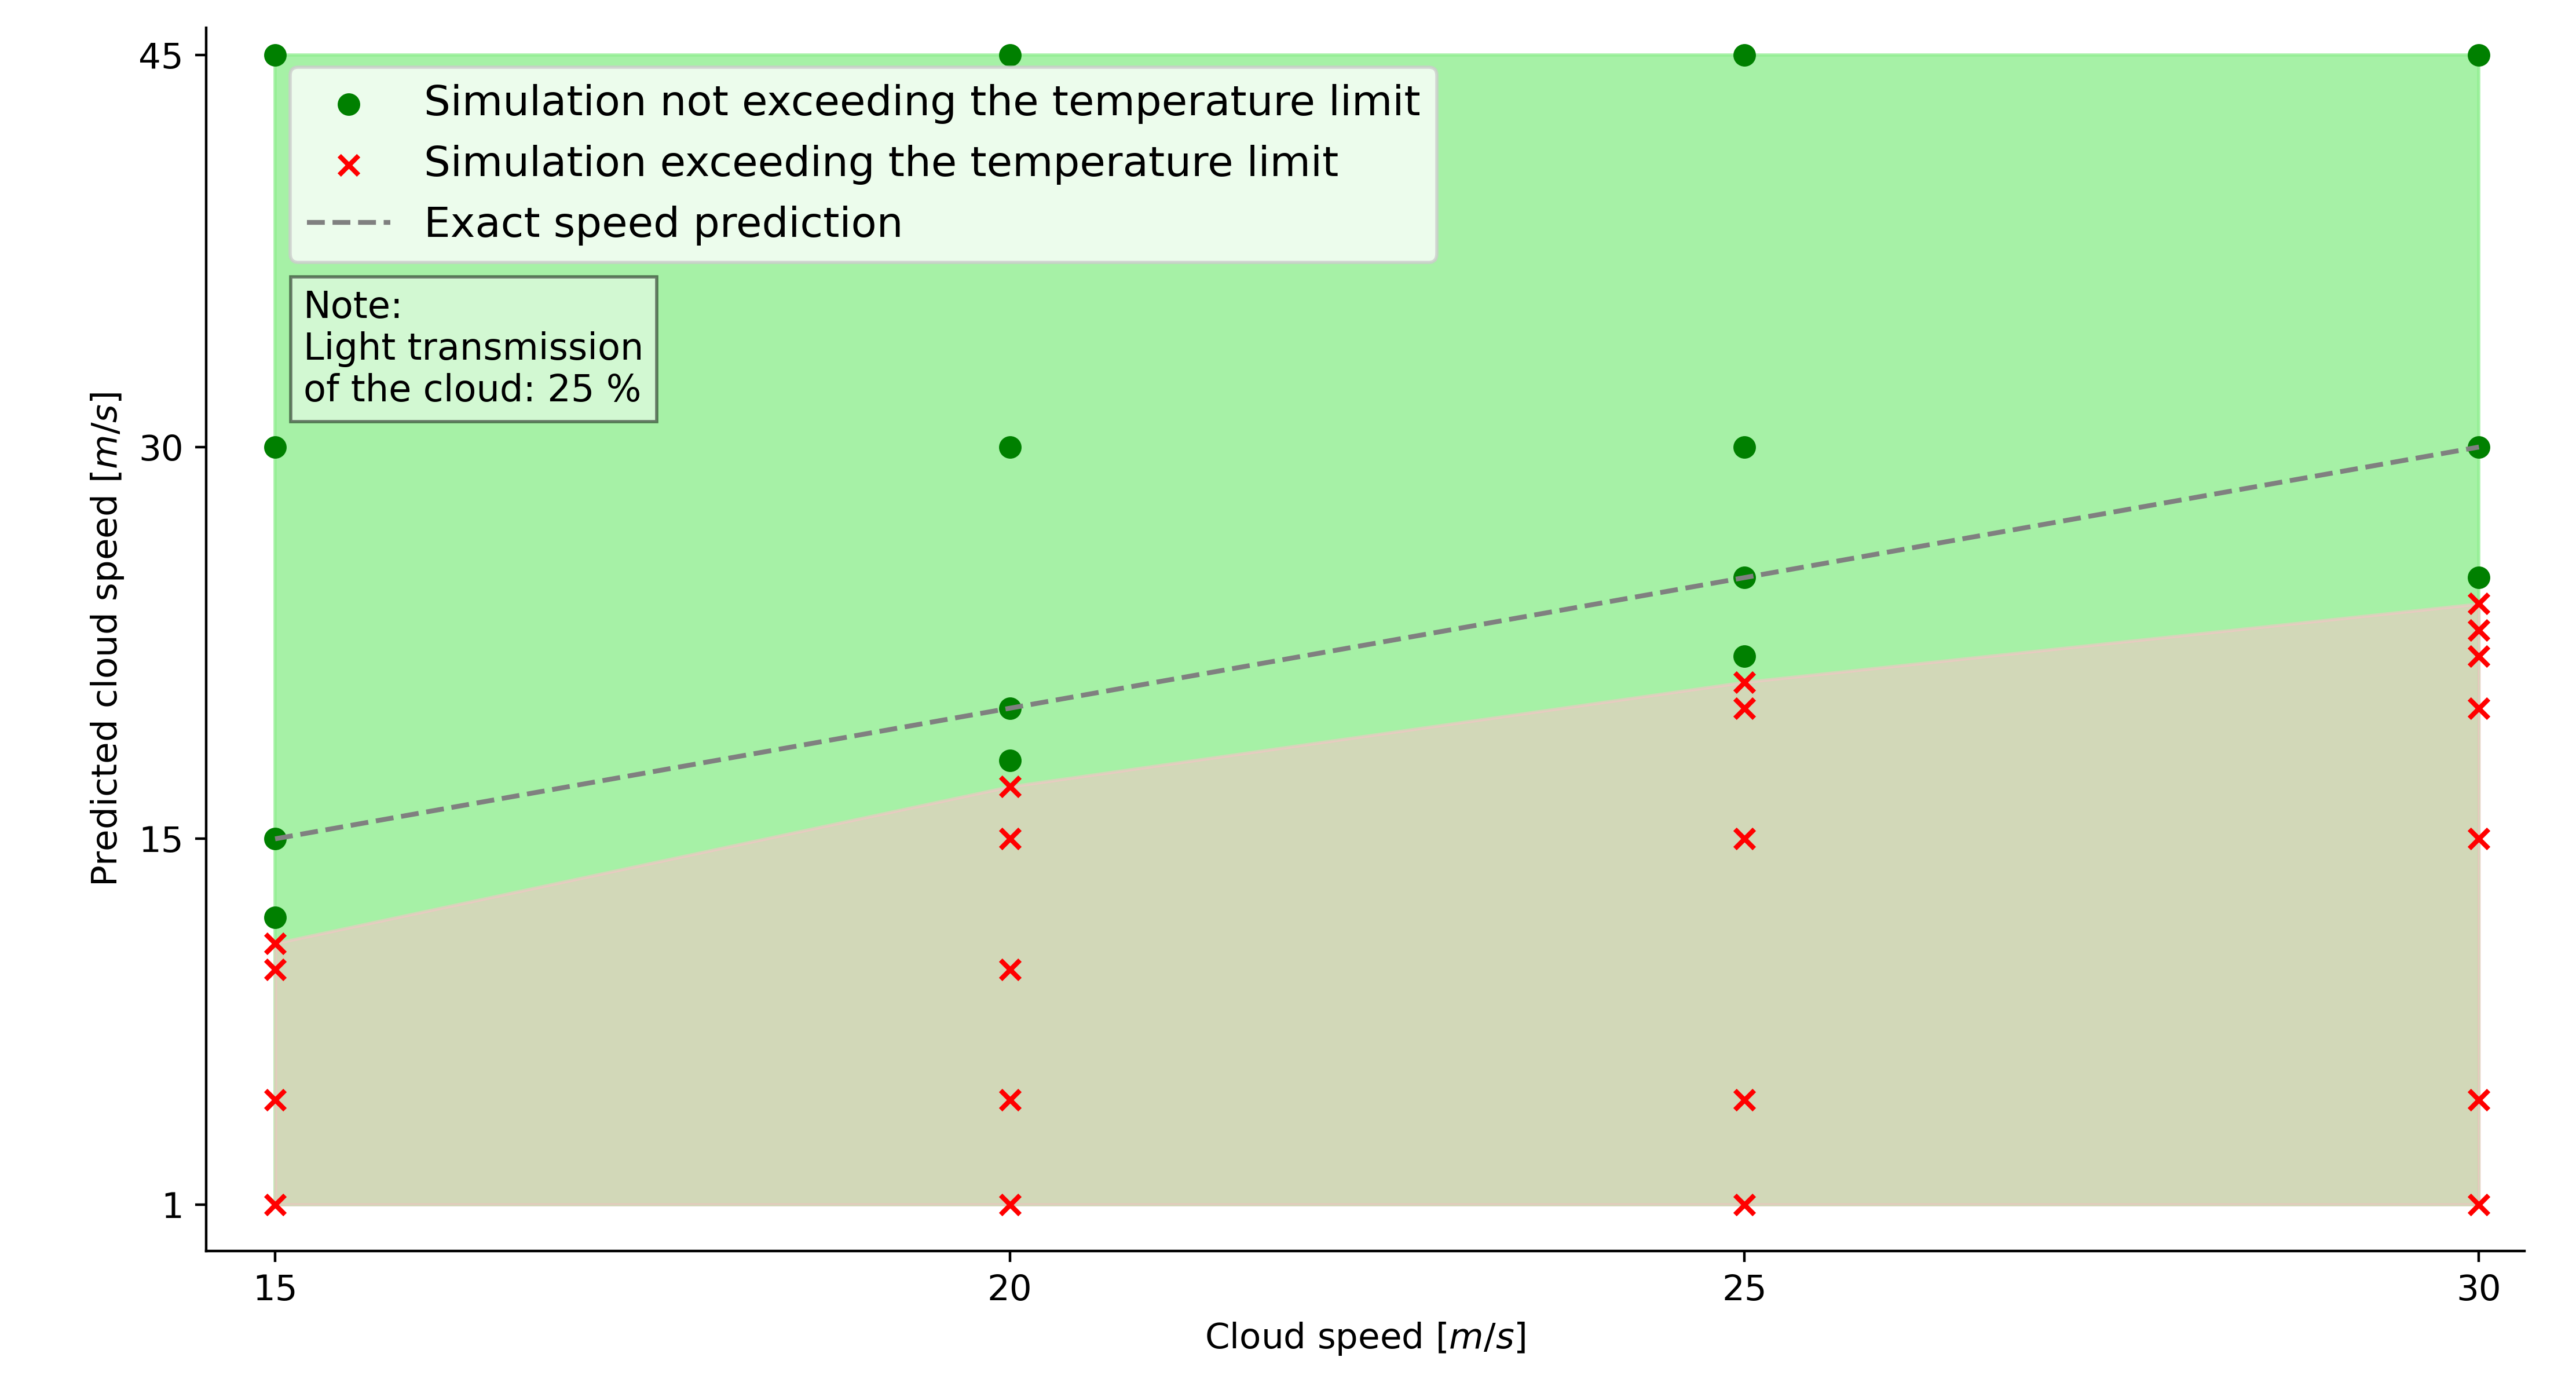
\includegraphics[width=0.99\textwidth]{C:/Users/gesc_ma/VSCode MPC Projekt/dynaovrcontroller/dynaovrcontroller/aimpoint_control_scenarios/plots/21_analyze_speed_uncertainty/safe_simulations_shading_25.png}}
    \caption[Analyse der erlaubten Abweichung in der Prädiktion der Wolkengeschwindigkeit für die Lichtdurchlässigkeit von $\SI{25}{\percent}$]{Analyse der erlaubten Abweichung in der Prädiktion der Wolkengeschwindigkeit für die Lichtdurchlässigkeit von $\SI{25}{\percent}$}
    \label{fig_speed25}
\end{figure}

Es ist ersichtlich, dass für diese Abschattung eine präzise Vorhersage der Wolkengeschwindigkeit notwendig ist.
Bei der Wolkengeschwindigkeit von $\SI{20}{\metre\per\second}$ darf die Vorhersage $\SI{18}{\metre\per\second}$ nicht unterschreiten.
Dies entspricht einer maximal zulässigen Abweichung von $\SI{-11}{\percent}$.
Jedoch zeigt Abbildung \ref{fig_speed25} auch, dass die vorhergesagte Wolkengeschwindigkeit die reale Geschwindigkeit durchaus überschreiten darf.
Grund dafür ist, dass eine schnellere Einstrahlungszunahme am Ende der Verschattungsdauer erwartet wird, als eigentlich auftritt.
Daher werden die Heliostaten schneller defokussiert und die maximale Fronttemperatur des Receivers wird nicht erreicht.
Dem gegenüber werden die Heliostaten zu langsam defokussiert, wenn die Wolkengeschwindigkeit höher ist vorhergesagt.
Beim Vergleich der Abbildung \ref{fig_speed25} mit den Analysen der ungenauen Geschwindigkeitsprädiktion für andere Einstrahlungsintensitäten (Abbildung \ref{fig_speed00} bis \ref{fig_speed75}) zeigt sich, dass die Vorhersage schnellerer Wolken in keinem der betrachteten Szenarien bedenklich ist.

Die Analyse der Temperaturabweichungen für die verschiedenen Geschwindigkeitsprädiktionen bei solarer Einstrahlung von $\SI{25}{\percent}$ zeigt Abbildung \ref{fig_speed25RMSE}.
Es wird deutlich, dass der RMSE zumeist geringer ist, je präziser die Wolkengeschwindigkeit vorhergesagt wurde.
Allerdings ist die Abweichung der Luftaustrittstemperatur für schneller vorhergesagte Wolken nur gering, wie an den erfolgreichen Simulationen zu erkennen ist.
Für die Wolkengeschwindigkeit von $\SI{25}{\metre\per\second}$ ist sogar zu sehen, dass bessere Ergebnisse bei schnellerer Geschwindigkeitsvorhersage auftreten können.
Dies ist auf mangelnde Konvergenz im Optimierungsprozess zurückzuführen, wenn 100 Iterationen überschritten werden (vgl. Kapitel \ref{sec_Hardsoftanalyse}).

\begin{figure}[h!]
    \centering
    \setlength{\fboxsep}{1pt}
    \setlength{\fboxrule}{1pt}
    \fbox{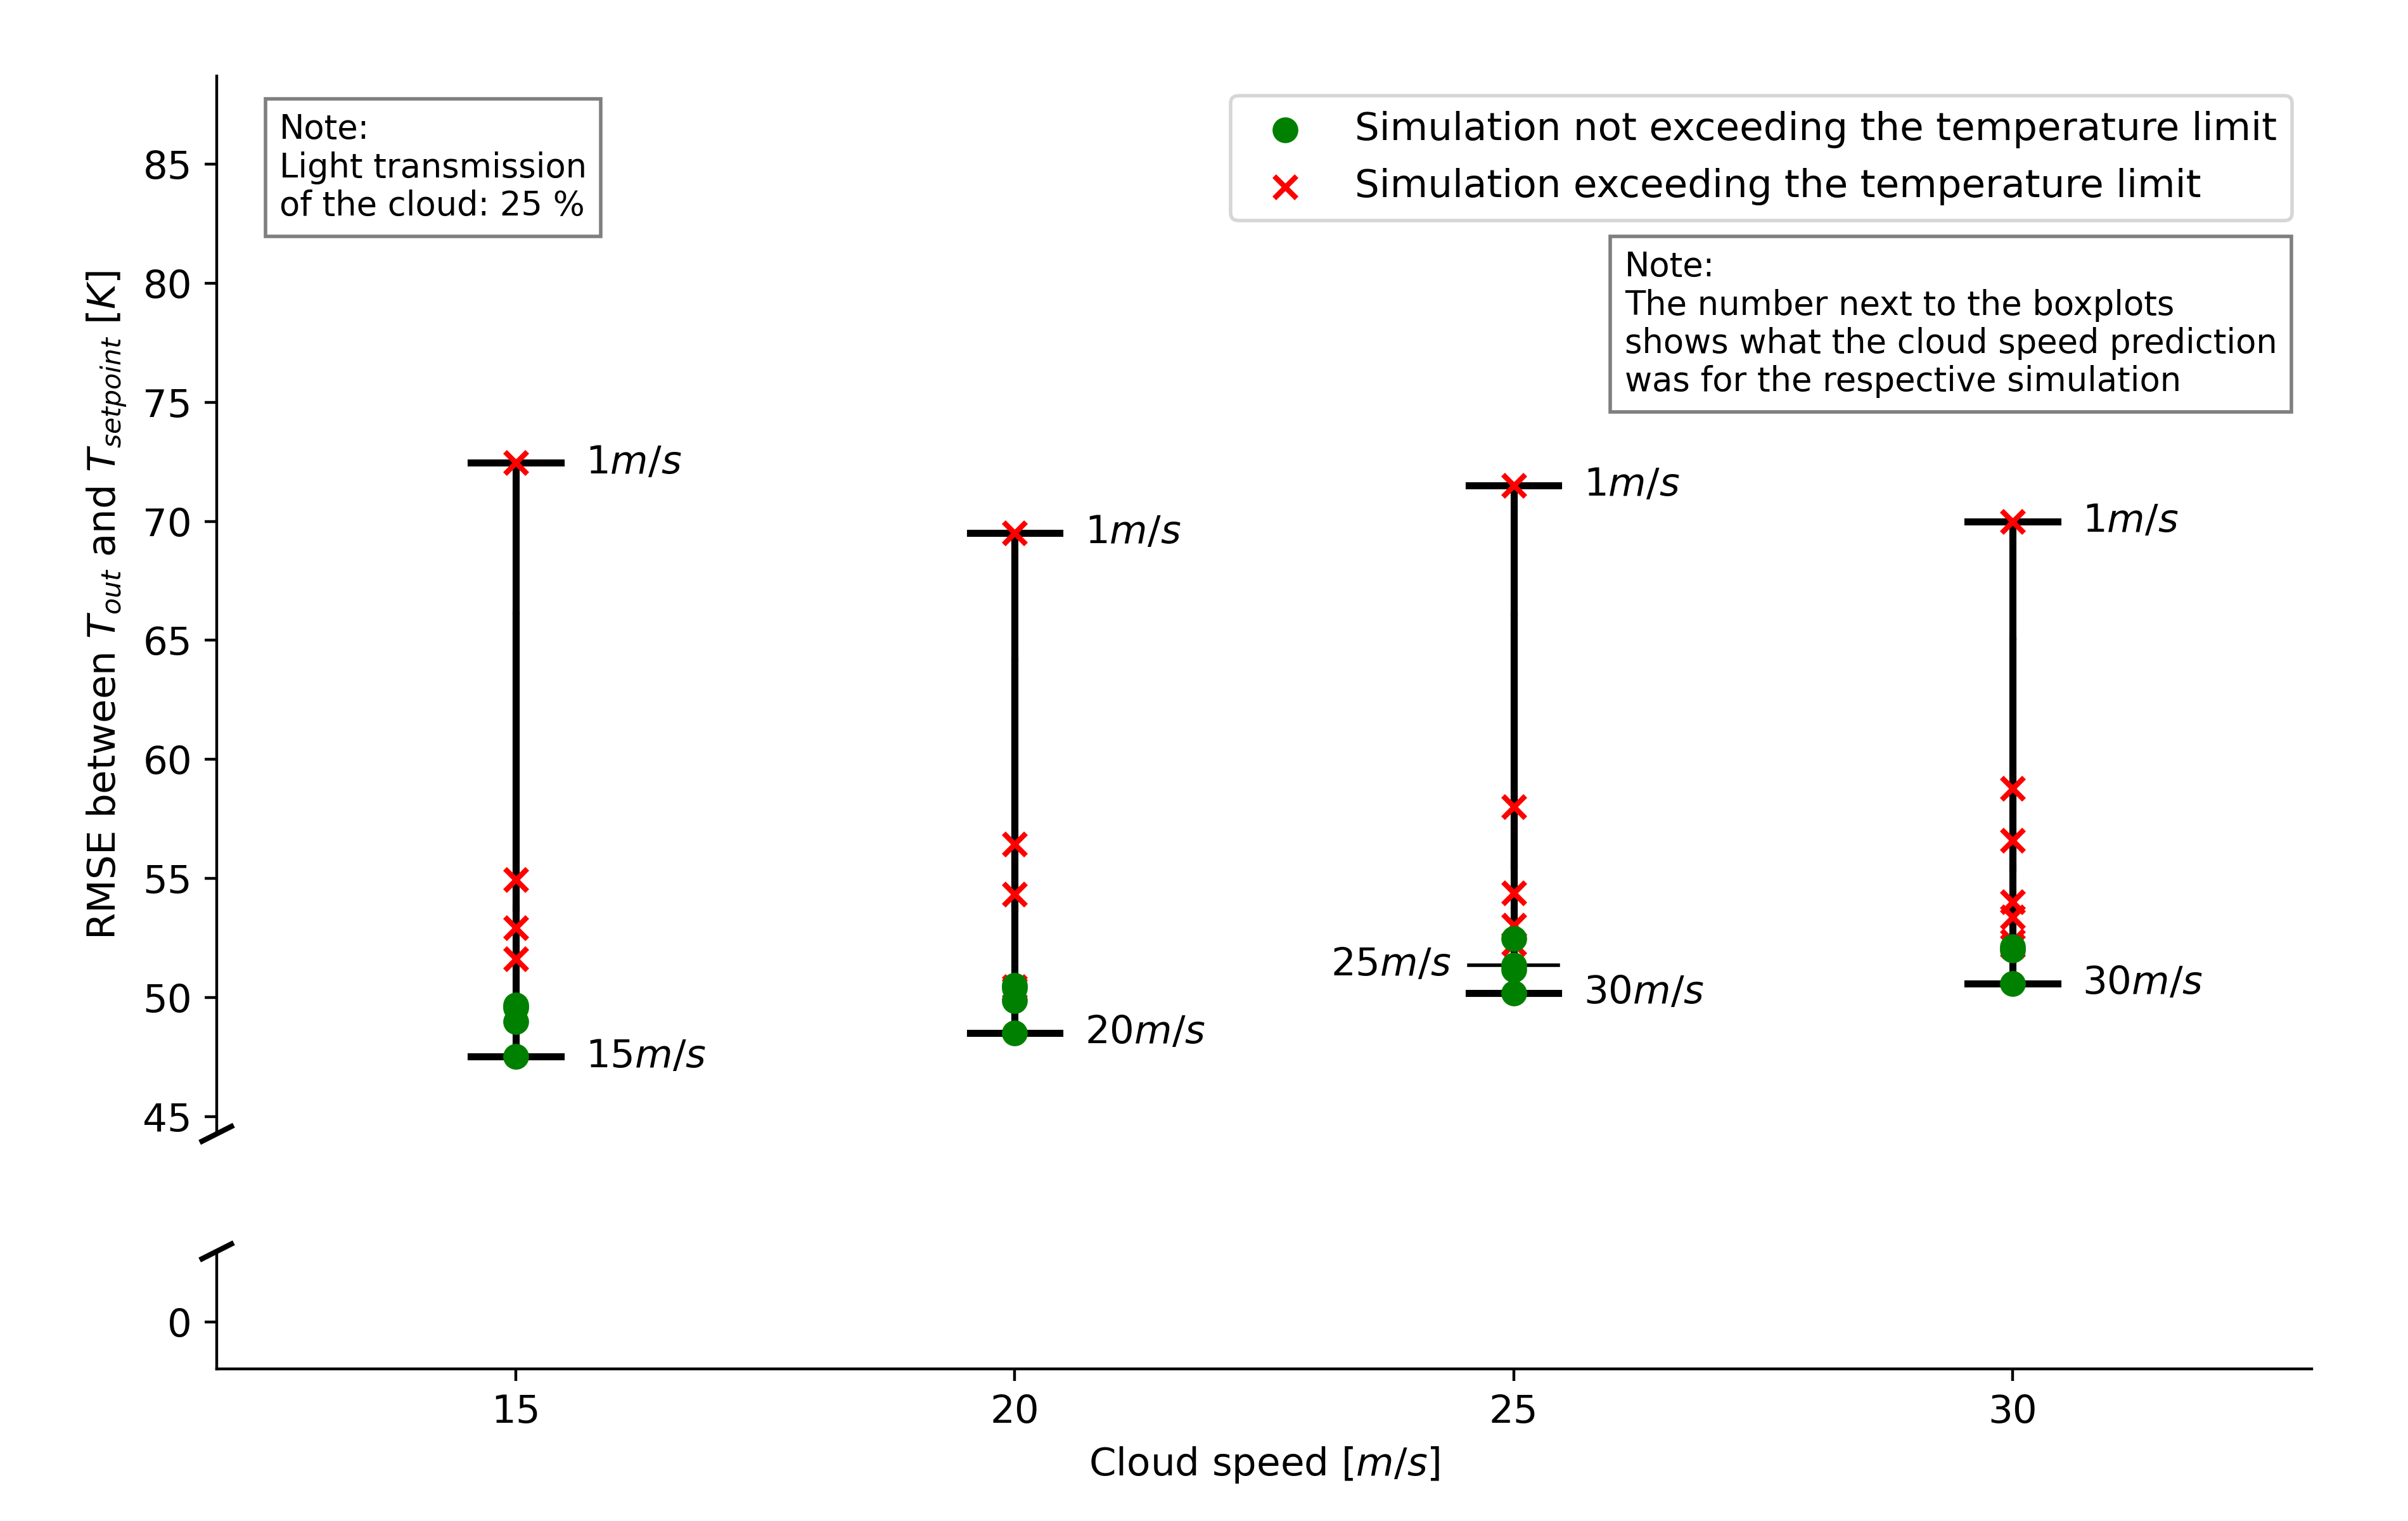
\includegraphics[width=0.99\textwidth]{C:/Users/gesc_ma/VSCode MPC Projekt/dynaovrcontroller/dynaovrcontroller/aimpoint_control_scenarios/plots/21_analyze_speed_uncertainty/rmse_per_speed_shading_25.png}}
    \caption[Analyse des RMSE für unterschiedliche Prädiktionen der Wolkengeschwindigkeiten für eine Lichtdurchlässigkeit der Wolke von $\SI{25}{\percent}$]{Analyse des RMSE für unterschiedliche Prädiktionen der Wolkengeschwindigkeiten für eine Lichtdurchlässigkeit der Wolke von $\SI{25}{\percent}$}
    \label{fig_speed25RMSE}
\end{figure}

Die Auswertungen des RMSE für die weiteren Verschattungsintensitäten (Abbildung \ref{fig_speed00RMSE} bis \ref{fig_speed75RMSE}) zeigen ebenfalls, dass die Vorhersage leicht höherer Wolkengeschwindigkeiten auch bezüglich des RMSE unproblematisch ist.
Daraus lässt sich schlussfolgern, dass die Prädiktion der Wolkengeschwindigkeit durch das Nowcasting eine Abweichung von $\SI{-11}{\percent}$ nicht unterschreiten darf.
Schnellere Wolkenvorhersagen resultieren ebenfalls in betriebssicheren Ergebnissen und nur geringfügig höherer Temperaturabweichung.


\subsection{Vorhersageungenauigkeit der Lichtdurchlässigkeit der Wolken} \label{subsec_shadingpräd}
Analog zur Wolkengeschwindigkeit in Abschnitt \ref{subsec_speedpräd} ist auch die fehlerfreie Vorhersage der Verschattungsintensität der Wolken nicht immer möglich.
Diese Prädiktionsabweichungen können dazu führen, dass eine stärkere Fokussierung der Heliostaten eingestellt wird, als es die reale solare Einstrahlung erfordert.
Im schlechtesten Fall kann dies ebenfalls dazu führen, dass die thermischen Belastungsgrenzen des Receivers überschritten werden.
Nachfolgend wird der Einfluss fehlerhaft vorhergesagter Verschattungsintensitäten auf die Sicherheit des Receivers untersucht, sowie der RMSE der Temperaturabweichung für diese Simulationsszenarien.

In Abbildung \ref{fig_shadingsafe} ist dargestellt, wie gut die Verschattungsvorhersage bei der maximalen betrachteten Wolkengeschwindigkeit von $\SI{30}{\metre\per\second}$ sein muss, damit die Grenztemperatur des Receivers eingehalten wird.
Es zeigt sich, dass bei einer Verschattung von $\SI{50}{\percent}$ eine besonders präzise Vorhersage der Abschattung erforderlich ist.
Wie in Kapitel \ref{sec_AllwissendeMPC} aufgezeigt, ist dies der Bereich, in dem die Regelung durch Fokussierung der Heliostaten besonders effizient gegenüber dem CSS ist.
Der Verschattung des Heliostatenfeldes kann durch Konzentration der Zielpunkte weitestgehend entgegengewirkt werden.
Ist die Vorhersage der Abschattung jedoch mehr als $\SI{5}{\percent}$ zu gering, kann dies zu einer Überschreitung der Grenztemperatur führen.

\begin{figure}[h!]
    \centering
    \setlength{\fboxsep}{1pt}
    \setlength{\fboxrule}{1pt}
    \fbox{\includegraphics[width=0.99\textwidth]{C:/Users/gesc_ma/VSCode MPC Projekt/dynaovrcontroller/dynaovrcontroller/aimpoint_control_scenarios/plots/20_analyze_shading_uncertainty/safe_simulations.png}}
    \caption[Analyse der erlaubten Abweichung in der Prädiktion der Lichtdurchlässigkeit für die Lichtdurchlässigkeit von $\SI{30}{\metre\per\second}$]{Analyse der erlaubten Abweichung in der Prädiktion der Lichtdurchlässigkeit für die Lichtdurchlässigkeit von $\SI{30}{\metre\per\second}$}
    \label{fig_shadingsafe}
\end{figure}

Grund dafür, dass besonders schlechte Prädiktionen für die Lichtdurchlässigkeit von $\SI{25}{\percent}$ bis $\SI{75}{\percent}$ trotzdem zu Simulationen führen, bei denen die Grenztemperatur nicht überschritten wird, ist die fehlende Konvergenz in der Optimierung (vgl. Abschnitt \ref{sec_Hardsoftanalyse}).
Abbildung \ref{fig_uncertain753050} zeigt für die Lichtdurchlässigkeit von $\SI{75}{\percent}$, dass bei $\SI{50}{\percent}$ vorhergesagter Abschattung die Grenztemperatur des Receivers überschritten wird.
Es ist erkennbar, dass der Regler mit einer geringeren Abschattung rechnet und die Heliostaten zu stark fokussiert.
Bei einer vorhergesagten Abschattung von $\SI{0}{\percent}$ konvergiert die Optimierung nicht, sodass kaum Regelungsverhalten zu erkennen ist und die Grenztemperatur nicht überschritten wird (vgl. Abbildung \ref{fig_uncertain753000}).

\begin{figure}[h!]
    \centering
    \setlength{\fboxsep}{1pt}
    \setlength{\fboxrule}{1pt}
    \fbox{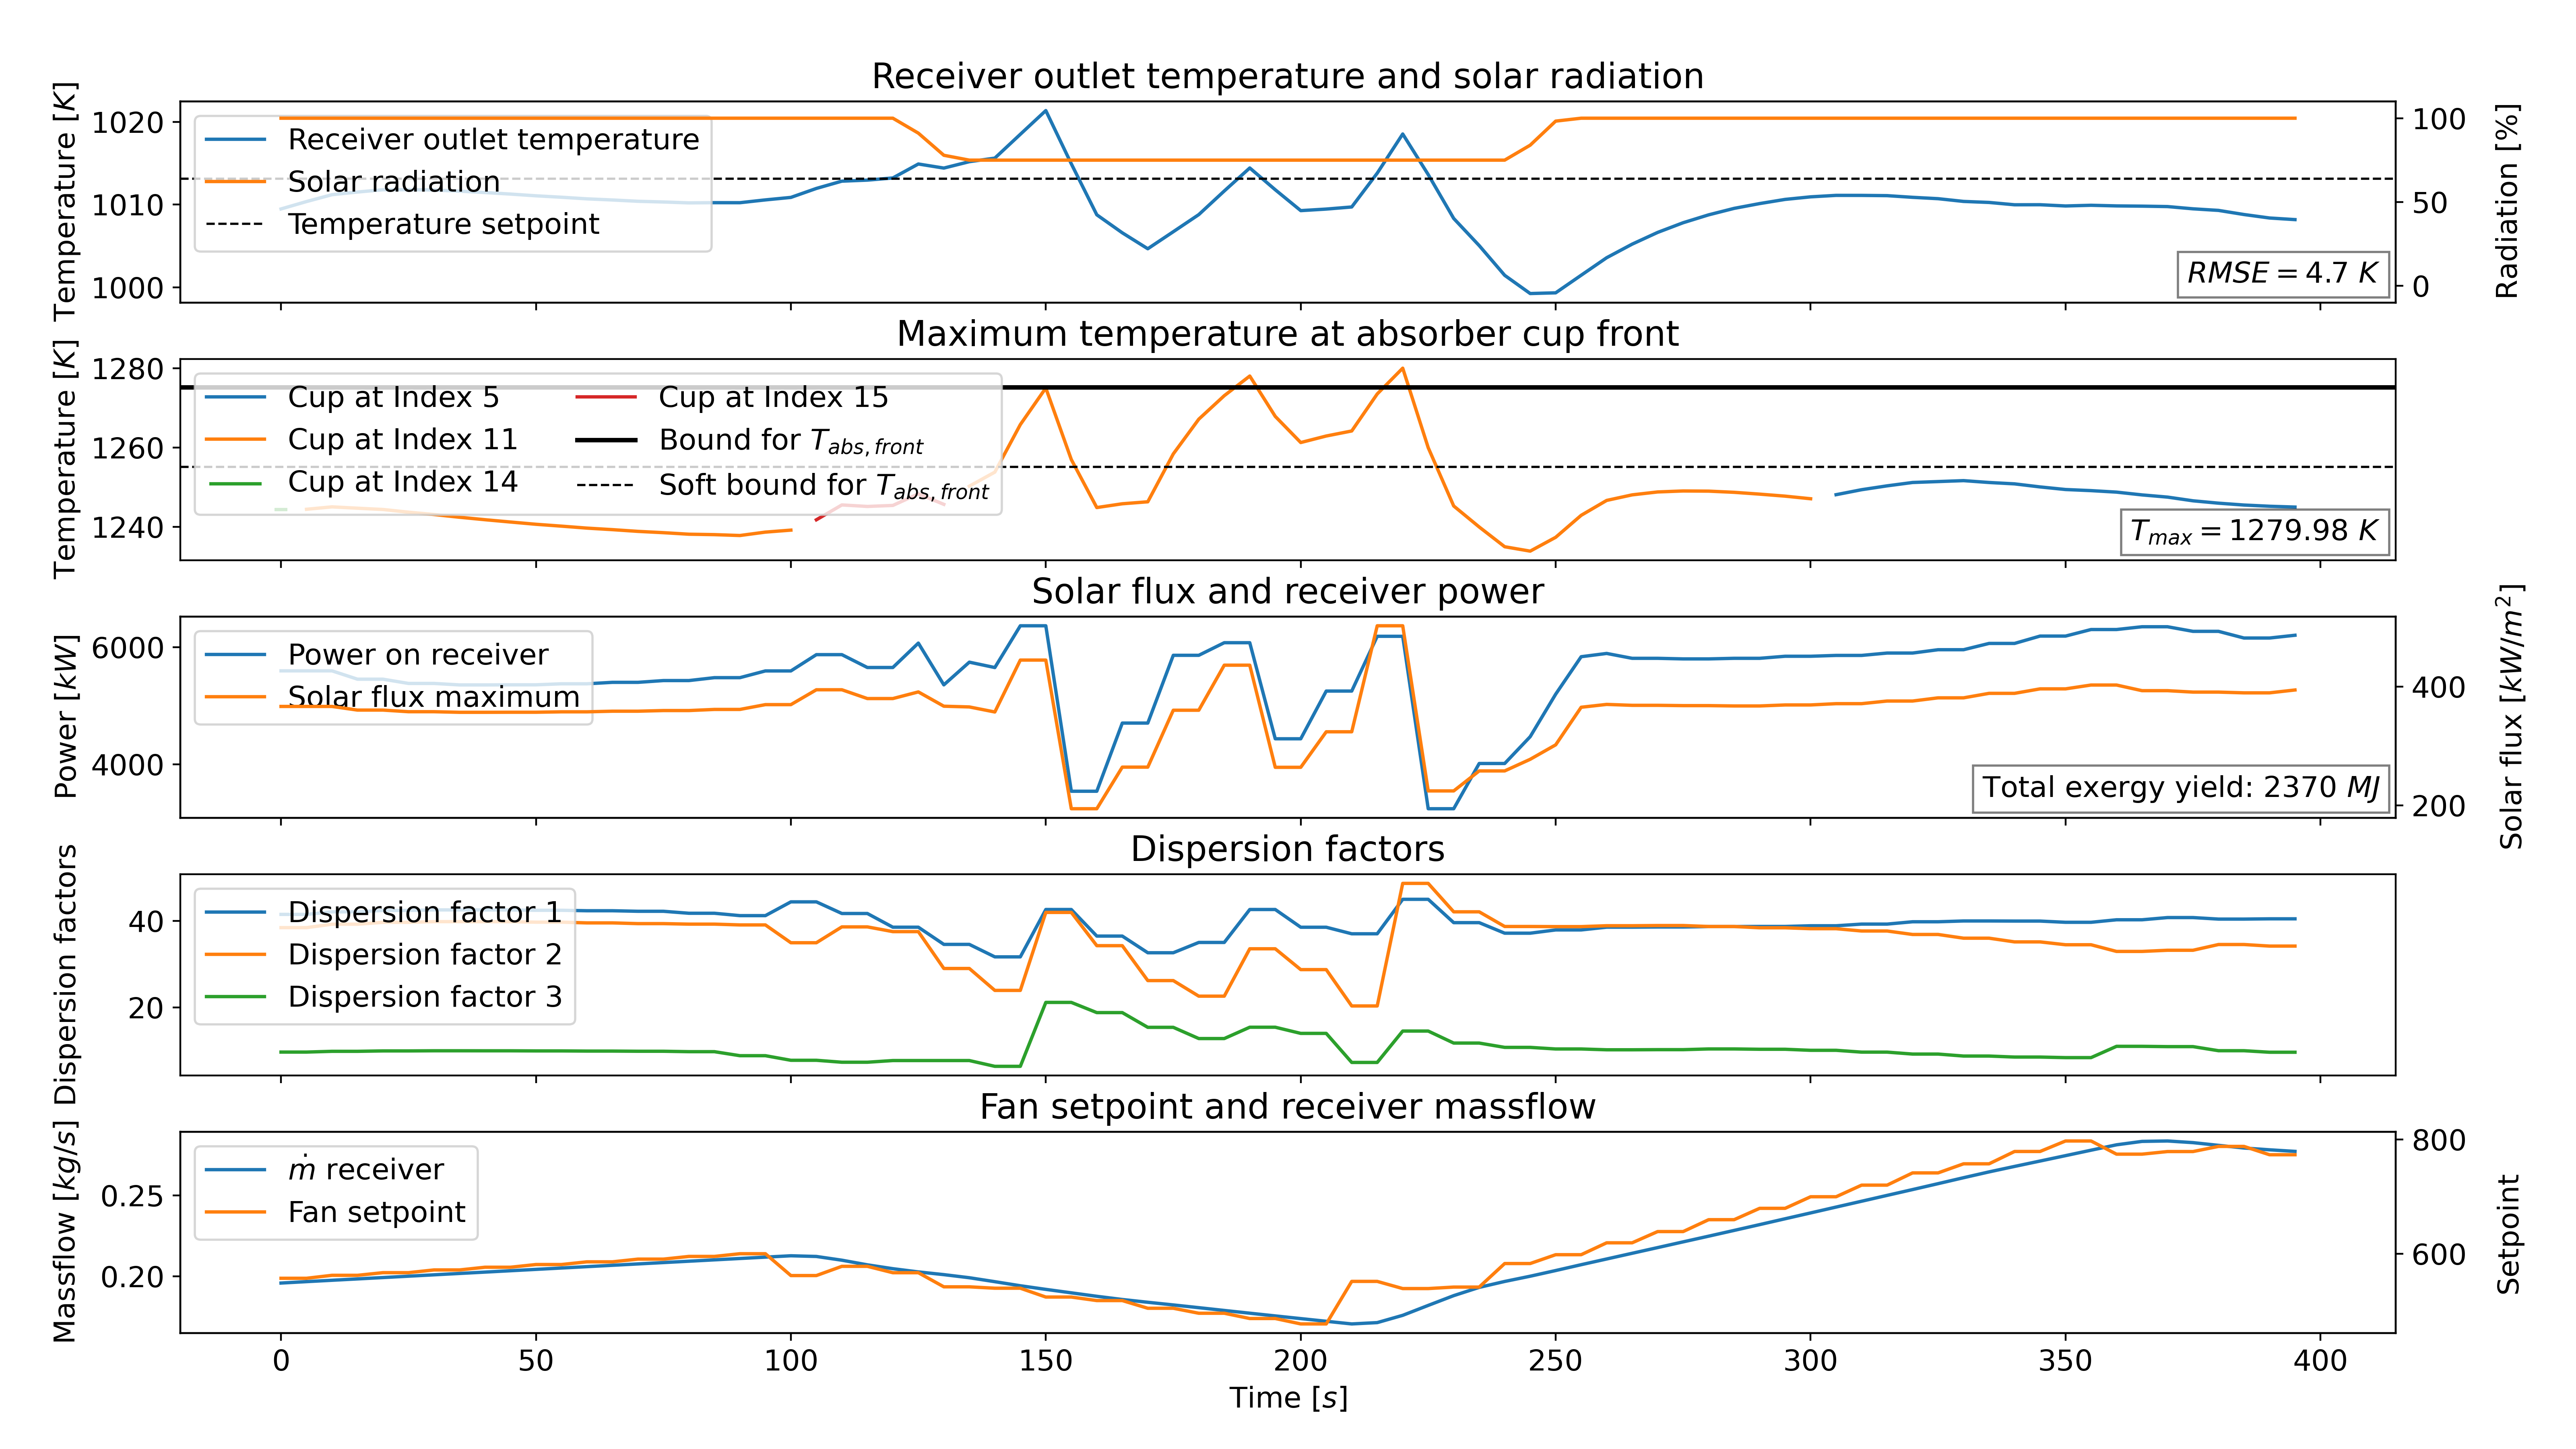
\includegraphics[width=0.99\textwidth]{C:/Users/gesc_ma/VSCode MPC Projekt/dynaovrcontroller/dynaovrcontroller/aimpoint_control_scenarios/plots/04_mpc_uncertain_information_shading/75/shading_120sec_75_30mps_thinking_50.png}}
    \caption[Simulationsverlauf mit Wolkengeschwindigkeit $\SI{30}{\metre\per\second}$ und Lichtdurchlässigkeit von $\SI{75}{\percent}$ bei Vorhersage von $\SI{50}{\percent}$]{Simulationsverlauf mit Wolkengeschwindigkeit $\SI{30}{\metre\per\second}$ und Lichtdurchlässigkeit von $\SI{75}{\percent}$ bei Vorhersage von $\SI{50}{\percent}$}
    \label{fig_uncertain753050}
\end{figure}

Bei Analyse des RMSE Verlaufes über die verschiedenen Abschattungen in Abbildung \ref{fig_shadingrmse} zeigt sich der in Kapitel \ref{sec_AllwissendeMPC} festgestellte, nahezu quadratische Zusammenhang zwischen Temperaturabweichung und Lichtdurchlässigkeit.
Es ist erkennbar, dass der RMSE bei starker Abschattung unabhängig von der Güte der Vorhersage über $\SI{100}{\kelvin}$ liegt.
Für andere Verschattungsszenarien ist die Temperaturabweichung geringer, wenn eine geringfügig schwächere Lichtdurchlässigkeit der Wolken prognostiziert wird, was Folge der unterschiedlichen optischen Modelle in der Modellbildung (vgl. Kapitel \ref{sec_optischesModell}) ist.

\begin{figure}[t]
    \centering
    \setlength{\fboxsep}{1pt}
    \setlength{\fboxrule}{1pt}
    \fbox{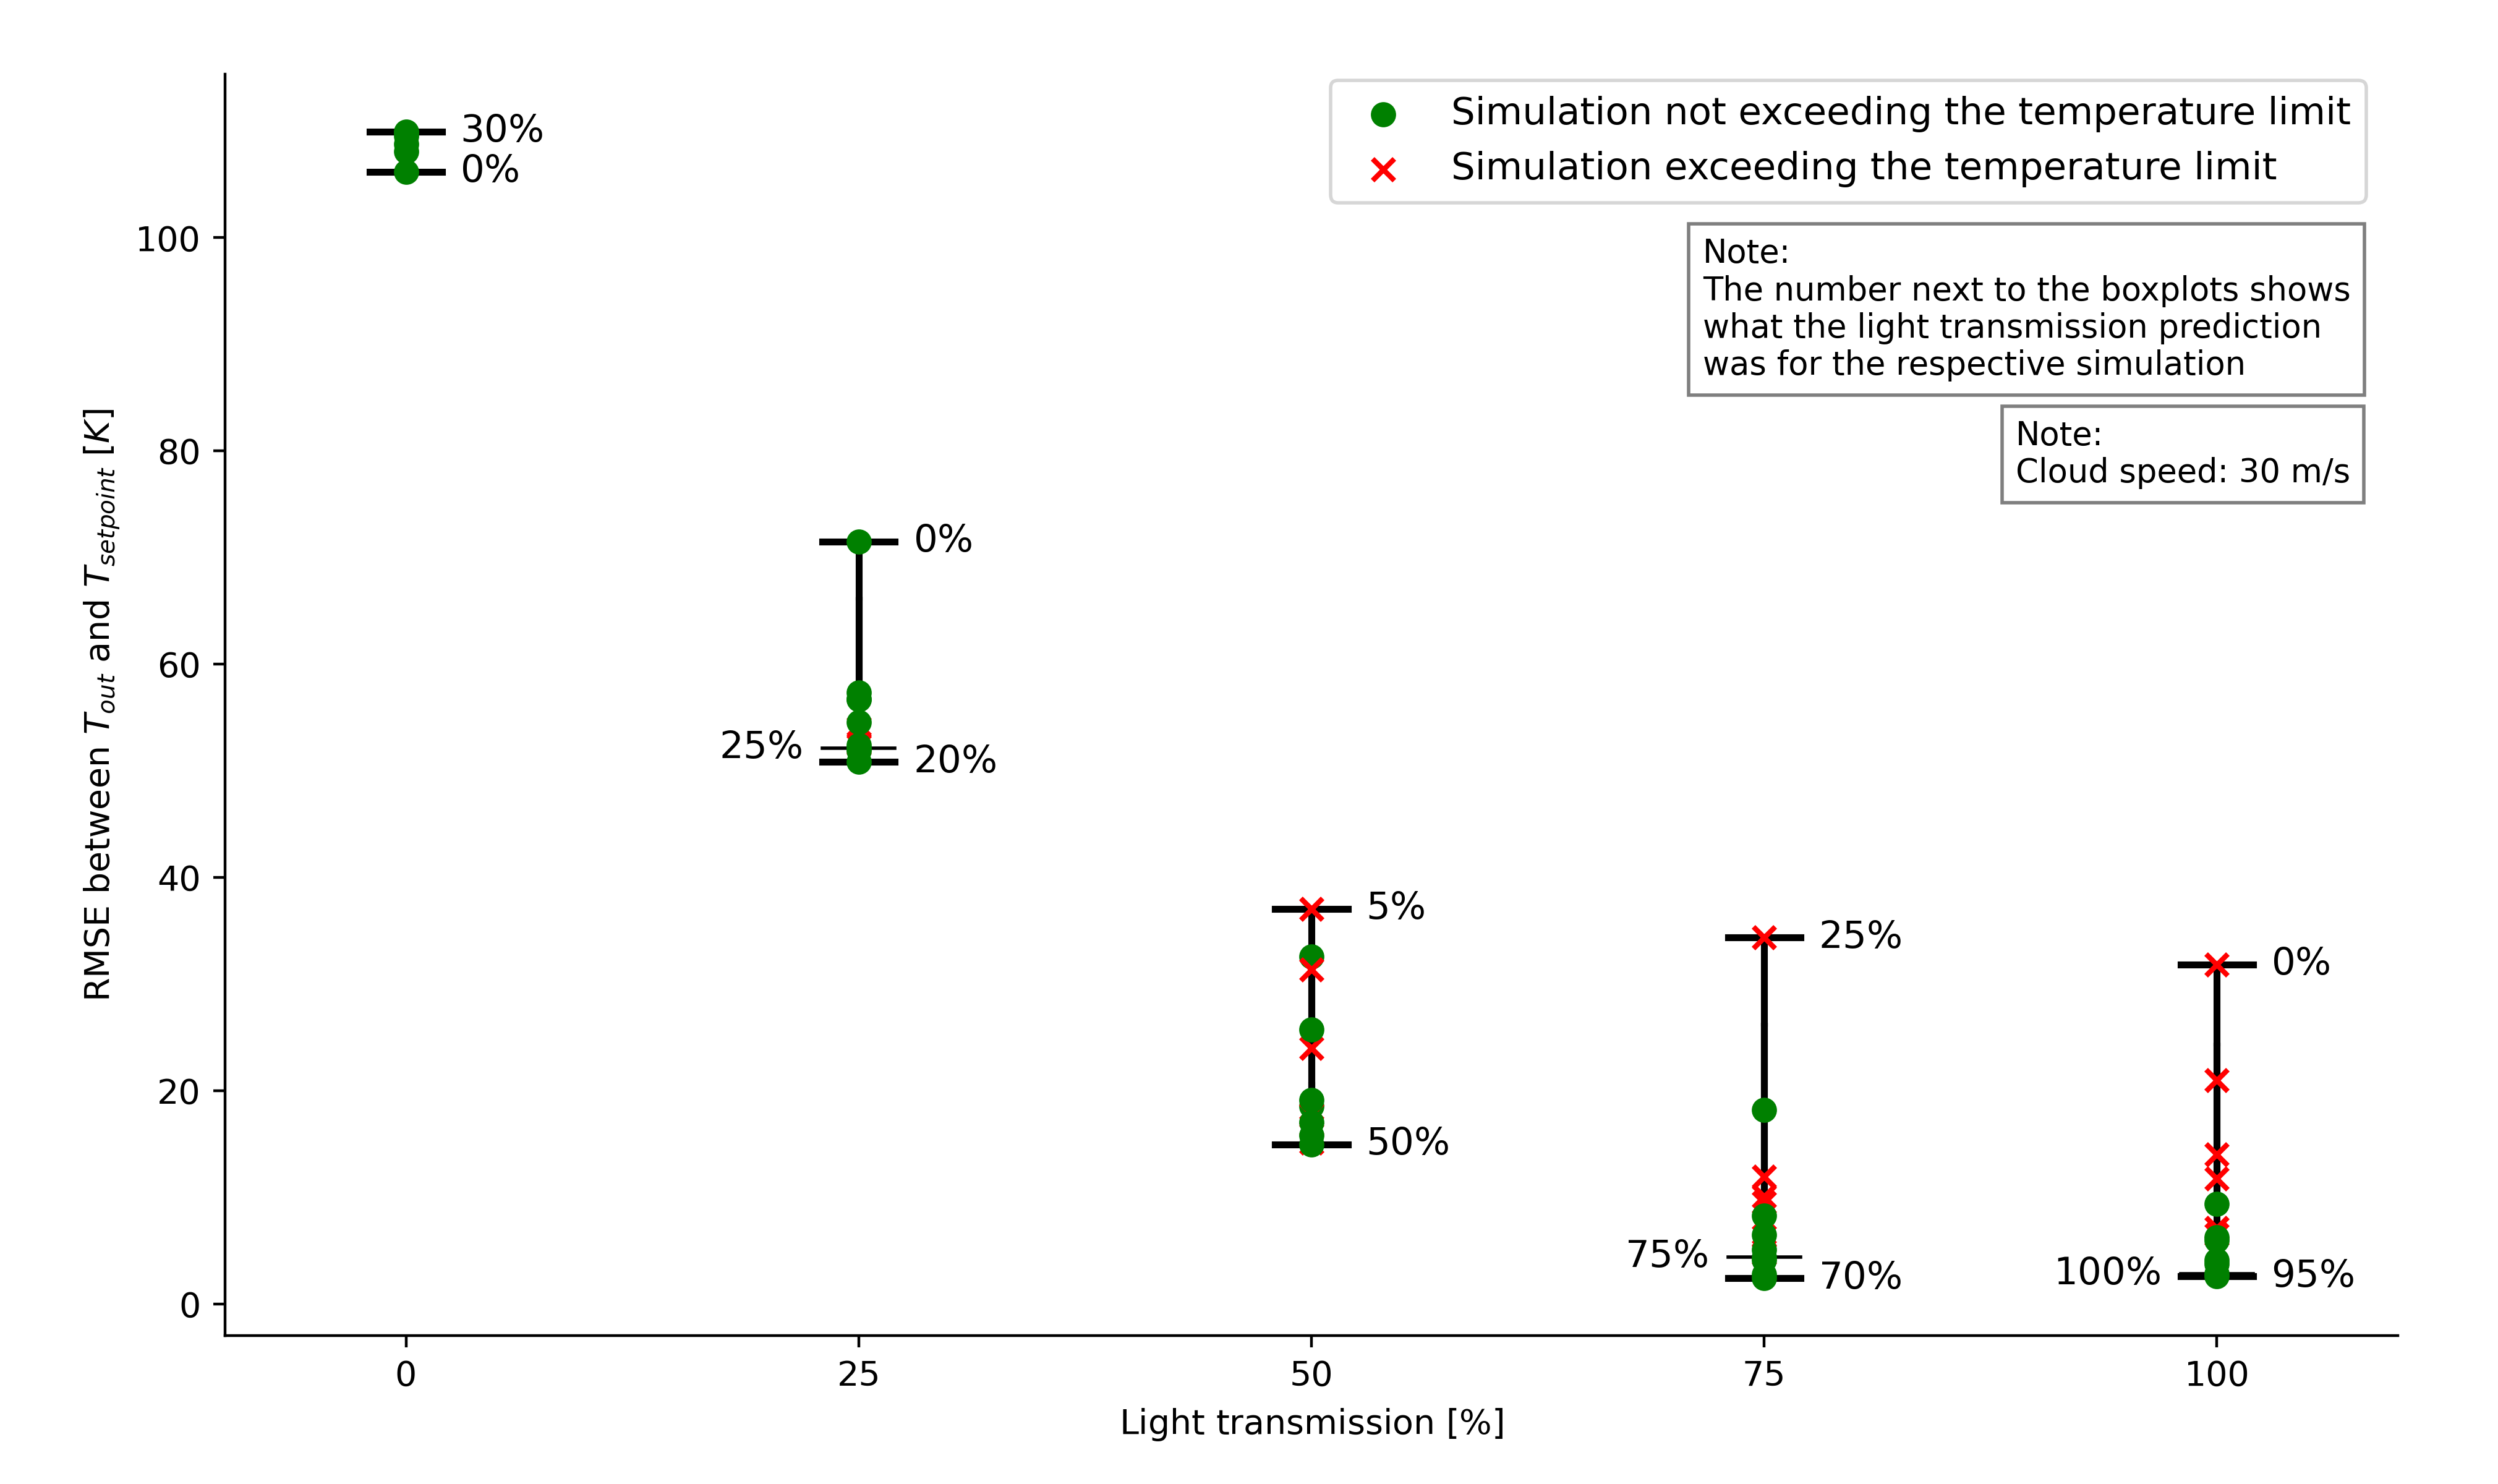
\includegraphics[width=0.99\textwidth]{C:/Users/gesc_ma/VSCode MPC Projekt/dynaovrcontroller/dynaovrcontroller/aimpoint_control_scenarios/plots/20_analyze_shading_uncertainty/rmse_per_shading.png}}
    \caption[Analyse des RMSE für unterschiedliche Prädiktionen der Verschattung für eine Wolkengeschwindigkeit von $\SI{30}{\metre\per\second}$]{Analyse des RMSE für unterschiedliche Prädiktionen der Verschattung für eine Wolkengeschwindigkeit von $\SI{30}{\metre\per\second}$}
    \label{fig_shadingrmse}
\end{figure}

Es zeigt sich, dass die Prädiktion des Nowcastings bezüglich der Lichtdurchlässigkeit der Wolken eine Genauigkeit von $\SI{>-5}{\percent}$ besitzen sollte.
Vorhersagen einer höheren Lichtdurchlässigkeit sind, analog zu der Vorhersage schnellerer Wolkengeschwindigkeiten, unproblematisch.
